%-------------------------------------------------------------------------
%-------------------------------------------------------------------------
%-------------------------------------------------------------------------

\chapter{Introduction}
\label{ch:Introduction}

%-------------------------------------------------------------------------
%-------------------------------------------------------------------------
%-------------------------------------------------------------------------

% \begin{epigraph}
%     \emph{It's a topsy-turvy world, and maybe the problems of two people don't amount to a hill of beans. But this is our hill. And these are our beans!} ---~Det. Lt. Frank Drebin (1988)
% \end{epigraph}

{\it Why do people visualize data?}

Ultimately, visualizing data allows people to consume\index{{\tt consume}} and produce\index{{\tt produce}} information in order to solve domain-specific problems or to communicate an understanding about phenomena relevant to a particular domain.
Visualization is often associated with data analysis and communication processes, however it is important to stress that not all data analysis and communication tasks are addressed via visualization.
This dissertation describes an approach that researchers and practitioners can use to systematically classify and abstract visualization tasks, whether they occur in a data analysis or communication context, and whether they involve the consumption or the production of information.
This abstraction of tasks is necessary and important because this abstraction facilitates visualization analysis and design: it can be used to communicate and transfer lessons learned from studying visualization tasks in specific application domains or with specific datatypes, it can be used to understand the implications of findings from controlled experiments, and it can be used to contextualize novel visualization techniques.

In this dissertation, we\footnote{With the exception of personal anecdotes in \autoref{intro:research-trajectory} and in the conclusion chapter, I will use the pronoun {\it we} throughout this dissertation to reflect the collaborative nature of the work reported therein.} present a typology\index{task!task typology} of abstract visualization tasks and document its application in three studies: in an interview study of individuals who visualize dimensionally reduced data in ten different application domains, in a post-deployment field study evaluation\index{evaluation} of a visual analysis tool in the domain of investigative journalism, and in a visualization design study\index{design studies} in the domain of energy management.
We also survey how our approach to task analysis\index{task!task analysis} has been adopted and extended by others visualization community.

%-------------------------------------------------------------------------
%-------------------------------------------------------------------------

\section{Research Trajectory}
\label{intro:research-trajectory}

%-------------------------------------------------------------------------
%-------------------------------------------------------------------------

Before discussing the contents and contributions of this dissertation in more detail, I will tell the story of how I came to study why people visualize data. 

When I entered my PhD program in late 2011, I posed the following question: {\it How do we evaluate visualization techniques and tools in an application domain context, particularly if these techniques and tools are used for data analysis?}\index{evaluation}
At this time, I read an early manuscript of a survey of visualization evaluation by \citet{Lam2012}, in which the authors read and coded over eight hundred recent visualization research papers that report an evaluation\index{evaluation} component.
While many of these papers discuss human perceptual performance or visualization usability, relatively few of these papers document an attempt to evaluate\index{evaluation} the use of visualization tools or techniques in settings other than in a controlled experiment, and fewer still comment on {\it adoption}\index{adoption}: whether a deployed visualization tool was incorporated into the recurring data analysis workflows of individuals working in a specific application domain.
The findings of this survey prompted me to ask: {\it Why is the study of real-world usage and adoption\index{adoption} of visualization techniques or tools reported so infrequently?} and {\it If this research is difficult to conduct, what makes it so difficult?}

Initially, I focused my study on the corpus of research papers emanating from the ACM \ac{BELIV} workshop series, where a number of methodologies and methods for evaluating\index{evaluation} visualization tools or techniques ``in the wild''\index{evaluation!in the wild} have been proposed. 
At the 2012 \ac{BELIV} workshop, there was substantial discussion pertaining to a need for a better shared understanding of the {\it tasks}\index{task} of people who visualize data or use visualization tools, and that the effective application of visualization evaluation\index{evaluation} methodologies depends upon this understanding.

My interest in evaluating\index{evaluation} visualization techniques and tools in real-world settings prompted me to undertake field study and a design study; both cases involved a visualization tool that was developed to address domain-specific problems.
In a design study, it is critical that the researchers have correctly abstracted the domain problems or use cases and mapped these to appropriate visual encoding\index{visual encoding} and interaction\index{interaction} design choices, perhaps incorporating design choices originally applied to other domains.
However, this abstraction and mapping is seldom straightforward: \citet{Sedlmair2012} describe how initial designs often fail to address the tasks\index{task} that people are expected to perform, how inappropriate evaluation\index{evaluation} methods are chosen, or how prematurely deployed visualization tools fail to be adopted\index{adoption} by the people for which they were designed.

By early 2013, my thinking had coalesced into a thesis statement expressed as follows: {\it visualization design and evaluation is difficult because mapping a person's tasks to visual encoding\index{visual encoding} and interaction\index{interaction} design choices requires multiple levels of abstraction. 
Researchers and practitioners would benefit from a domain-agnostic, consistent, and validated approach for assisting in this mapping}.

\bqstart{What is a ``task''?}
A {\it task}\index{task} is an ill-defined concept, and as the reader will discover in \autoref{ch:typology}, there is currently little agreement in the visualization literature as to the appropriate granularity for describing a task\index{task}.
For instance, {\it finding an extreme value}~\cite{Amar2005} is less abstract than {\it exploring}~\cite{Yi2007}\index{{\tt explore}} or {\it integrating insights}\index{insight}~\cite{Springmeyer1992}, while {\it comparing sequence variants in a human genome}\index{{\tt compare}} is quite domain-specific.
This confusion is the result of a conflation of two axes on which we might characterize a task: level of abstraction\index{task!task abstraction} and applicability\index{task!task applicability}, in which the latter refers to the specificity of a task\index{task} with respect to a particular application domain or datatype.
% RR:p. 3. "exploring [234] or integrating insights [188] are quite abstract". Do you really mean "abstract", or do you mean "vague"? (cf. discussion of "exploring" on p. 11.) Related to this: couldn't "finding an extreme value" be abstract?  If not, what do you mean by "abstraction"? Isn't this simply independence of the details of the task?
Relating these task\index{task} descriptions is difficult, though not impossible; however, visualization practitioners hardly have a shared lexicon when describing these relations between levels of abstraction\index{task!task abstraction} and application\index{task!task applicability} areas.

Researchers and practitioners should strive to go beyond merely describing the use of visualization tools or techniques in a specific application domain; rather they should {\it abstract}\index{task!task abstraction} these domain-specific tasks\index{task} in order to realize an appropriate visualization design space.
This abstraction\index{task!task abstraction} also lets practitioners contribute back to the visualization research community, transferring their findings beyond a single domain. 

My dissertation examines visualization task abstraction\index{task!task abstraction} from multiple perspectives.
\autoref{ch:typology} documents the synthesis of related work classifying tasks\index{task}, interactions\index{interaction}, and visualization design choices.
The result of this synthesis was a new approach to task analysis\index{task!task analysis}, a typology\index{task!task typology} for classifying visualization tasks at multiple levels of abstraction.
However, proposing this typology\index{task!task typology} was not enough. 
We had to validate this typology\index{task!task typology} as a pragmatic tool~\cite{Beaudouin-Lafon2004}; to do so, we used the typology\index{task!task typology} to {\it describe} existing interactions\index{interaction} between people and visualization techniques or tools, to {\it generate} new designs, and to {\it evaluate}\index{evaluation} these designs.
The three forms of validation are intertwined, as the ability to {\it generate} or {\it evaluate}\index{evaluation} implies the ability to {\it describe}; in this dissertation, we address all three types of validation.

The remainder of this dissertation serves to validate this typology\index{task!task typology} in applied settings spanning multiple domains.
In \autoref{ch:drvistasks}, we used our typology\index{task!task typology} to {\it analyze} findings from an interview study spanning several different application domains, focusing on individuals who visualize dimensionally reduced\index{dimensionality reduction (DR)} data.
In \autoref{ch:overview}, we used our typology\index{task!task typology} in a field study to {\it evaluate}\index{evaluation} {\it Overview}\index{Overview (document mining tool)}, a visual analysis tool that was adopted\index{adoption} by investigative journalists.
Finally, in \autoref{ch:emu}, we used our typology\index{task!task typology} to {\it design} and evaluate\index{evaluation} visualization designs in the domain of energy management.

%-------------------------------------------------------------------------
%-------------------------------------------------------------------------

\section{Motivation}
\label{intro:motivation}

%-------------------------------------------------------------------------
%-------------------------------------------------------------------------

Task analysis\index{task!task analysis} is essential for visualization analysis, evaluation\index{evaluation}, and design.
While there are many approaches to visualization task analysis\index{task!task analysis}, they vary in terms of level of abstraction, applicability\index{task!task applicability} across domains and datatypes, as well as in terms of the vocabulary that they use. 
The visualization community requires a synthesis of existing task analysis\index{task!task analysis} approaches and theoretical foundations, one that spans multiple levels of abstraction, spans across domains and datatypes, and introduces a common and consistent task lexicon\footnote{We elaborate on this motivation in \autoref{ch:typology}}.

This dissertation demonstrates that such a synthesis is possible. 
Furthermore, we demonstrate our approach to task analysis\index{task!task analysis} in visualization analysis, evaluation\index{evaluation}, and design projects.
We also report on the adoption of our approach by others in the community.

%-------------------------------------------------------------------------
%-------------------------------------------------------------------------

\section{Thesis Contributions}
\label{intro:research-program}

%-------------------------------------------------------------------------
%-------------------------------------------------------------------------

There are four research chapters contained in this dissertation, each offering contributions to the visualization research community.
A succinct summary of all contributions appears at the end of this section.

%-------------------------------------------------------------------------

\subsection{A Typology of Abstract Visualization Tasks}
\label{intro:p1}

%-------------------------------------------------------------------------

The visualization design and evaluation process is characterized by multiple levels~\cite{Munzner2009, Munzner2014}, as characterized by Munzner's nested model\index{nested model (Munzner)}, shown in see \autoref{fig:nested-model}.
These levels include the domain problem, data and task abstractions\index{task!task abstraction}, visual encoding\index{visual encoding} and interaction\index{interaction} design choices, and ultimately the algorithms\index{algorithms} that drive them.
In this dissertation, our focus is on task abstractions\index{task!task abstraction}, how they map upward to domain problems, and how they map downward to visualization design choices.

%-|-|-|-|-|-|-|-|-|-|-|-|-|-|-|-|-|-|-|-|-|-|-|-|-|-|-|-|-|-|-|-|-|-|-|-|-

\begin{figure}
	\centering
    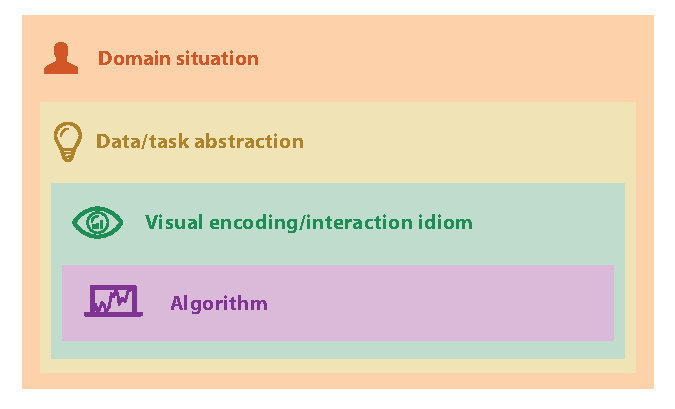
\includegraphics[width=0.75\textwidth]{figures/fig4-2.pdf}
    \caption
    [
        Munzner's nested model of visualization design.
    ]
    {
        Munzner's nested model of visualization design~\cite{Munzner2009,Munzner2014}; the arrows indicate the cascading effects of design decisions made at higher levels. Illustration: \ccLogo~E. Maguire (2014).
    }
	\centering
	\label{fig:nested-model}
\end{figure}

%-|-|-|-|-|-|-|-|-|-|-|-|-|-|-|-|-|-|-|-|-|-|-|-|-|-|-|-|-|-|-|-|-|-|-|-|-

As indicated in \autoref{intro:research-trajectory}, my personal motivation for developing an approach for classifying and abstracting tasks\index{task!task abstraction} was pragmatic: we had amassed observational data of the use of visualization tools and techniques in the interview study and field study projects, described in \autoref{ch:drvistasks} and \autoref{ch:overview} respectively, where we struggled to describe and compare tasks\index{task} performed by different people, tasks\index{task} performed with different visualization techniques or tools, as well as tasks\index{task} associated with different application domains.
We required a systematic approach for analyzing tasks\index{task!task analysis} abstractly\index{task!task abstraction}, allowing us to describe and evaluate\index{evaluation} visualization design choices that address these tasks.

\bstart{Methodology}
In \autoref{ch:typology}, we describe our comprehensive review of previous work that classified tasks\index{task}, interactions\index{interaction}, activities, and visualization design choices.
This review included over two dozen previous classification systems and theoretical frameworks from the literatures of visualization, \ac{HCI}\index{human-computer interaction (HCI)}, information retrieval\index{information retrieval}, communications\index{communications}, and cartography\index{cartography}. 
We examined the vocabulary and definitions used in this body of previous work, and after multiple rounds of coding\index{coding (qualitative data analysis)}, we had grouped similar terms, determined representative terms for each group, and arranged these representative terms into multiple levels of abstraction\footnote{\autoref{app:typology} documents the evolution of our typology.}.
We reasoned about how tasks could be described using this arrangement of terms, either in isolation, or as a sequence of interdependent tasks\index{task!task sequence}.

\bstart{Contributions}
The result of our synthesis was a typology\index{task!task typology} of abstract visualization tasks\index{task!task abstraction}, illustrated in \autoref{fig:typology}.
This typology\index{task!task typology} allows for succinct descriptions of tasks, in which a task description is comprised of {\it why}\index{{\tt why}} data is visualized (at multiple levels of abstraction), {\it what}\index{{\tt what}} dependencies a task might have in terms of {\it input}\index{{\tt input}} and {\it output}\index{{\tt output}}, and {\it how}\index{{\tt how}} the task is or can be supported in terms of visual encoding\index{visual encoding} and interaction\index{interaction} design choices; given this structure, it is possible to describe sequences of interdependent tasks\index{task!task sequence}, as illustrated in \autoref{fig:typology-dep} and in the example of \autoref{fig:typology-example}.
Our typology\index{task!task typology} has since proven to be useful in our subsequent interview study (\autoref{ch:drvistasks}), field study (\autoref{ch:overview}), and design study (\autoref{ch:emu}) projects, as well as in recent work by others; we reflect upon the adaptation and use of our typology\index{task!task typology} by others in \autoref{ch:conclusions}.

%-|-|-|-|-|-|-|-|-|-|-|-|-|-|-|-|-|-|-|-|-|-|-|-|-|-|-|-|-|-|-|-|-|-|-|-|-

\begin{figure}
    \centering
    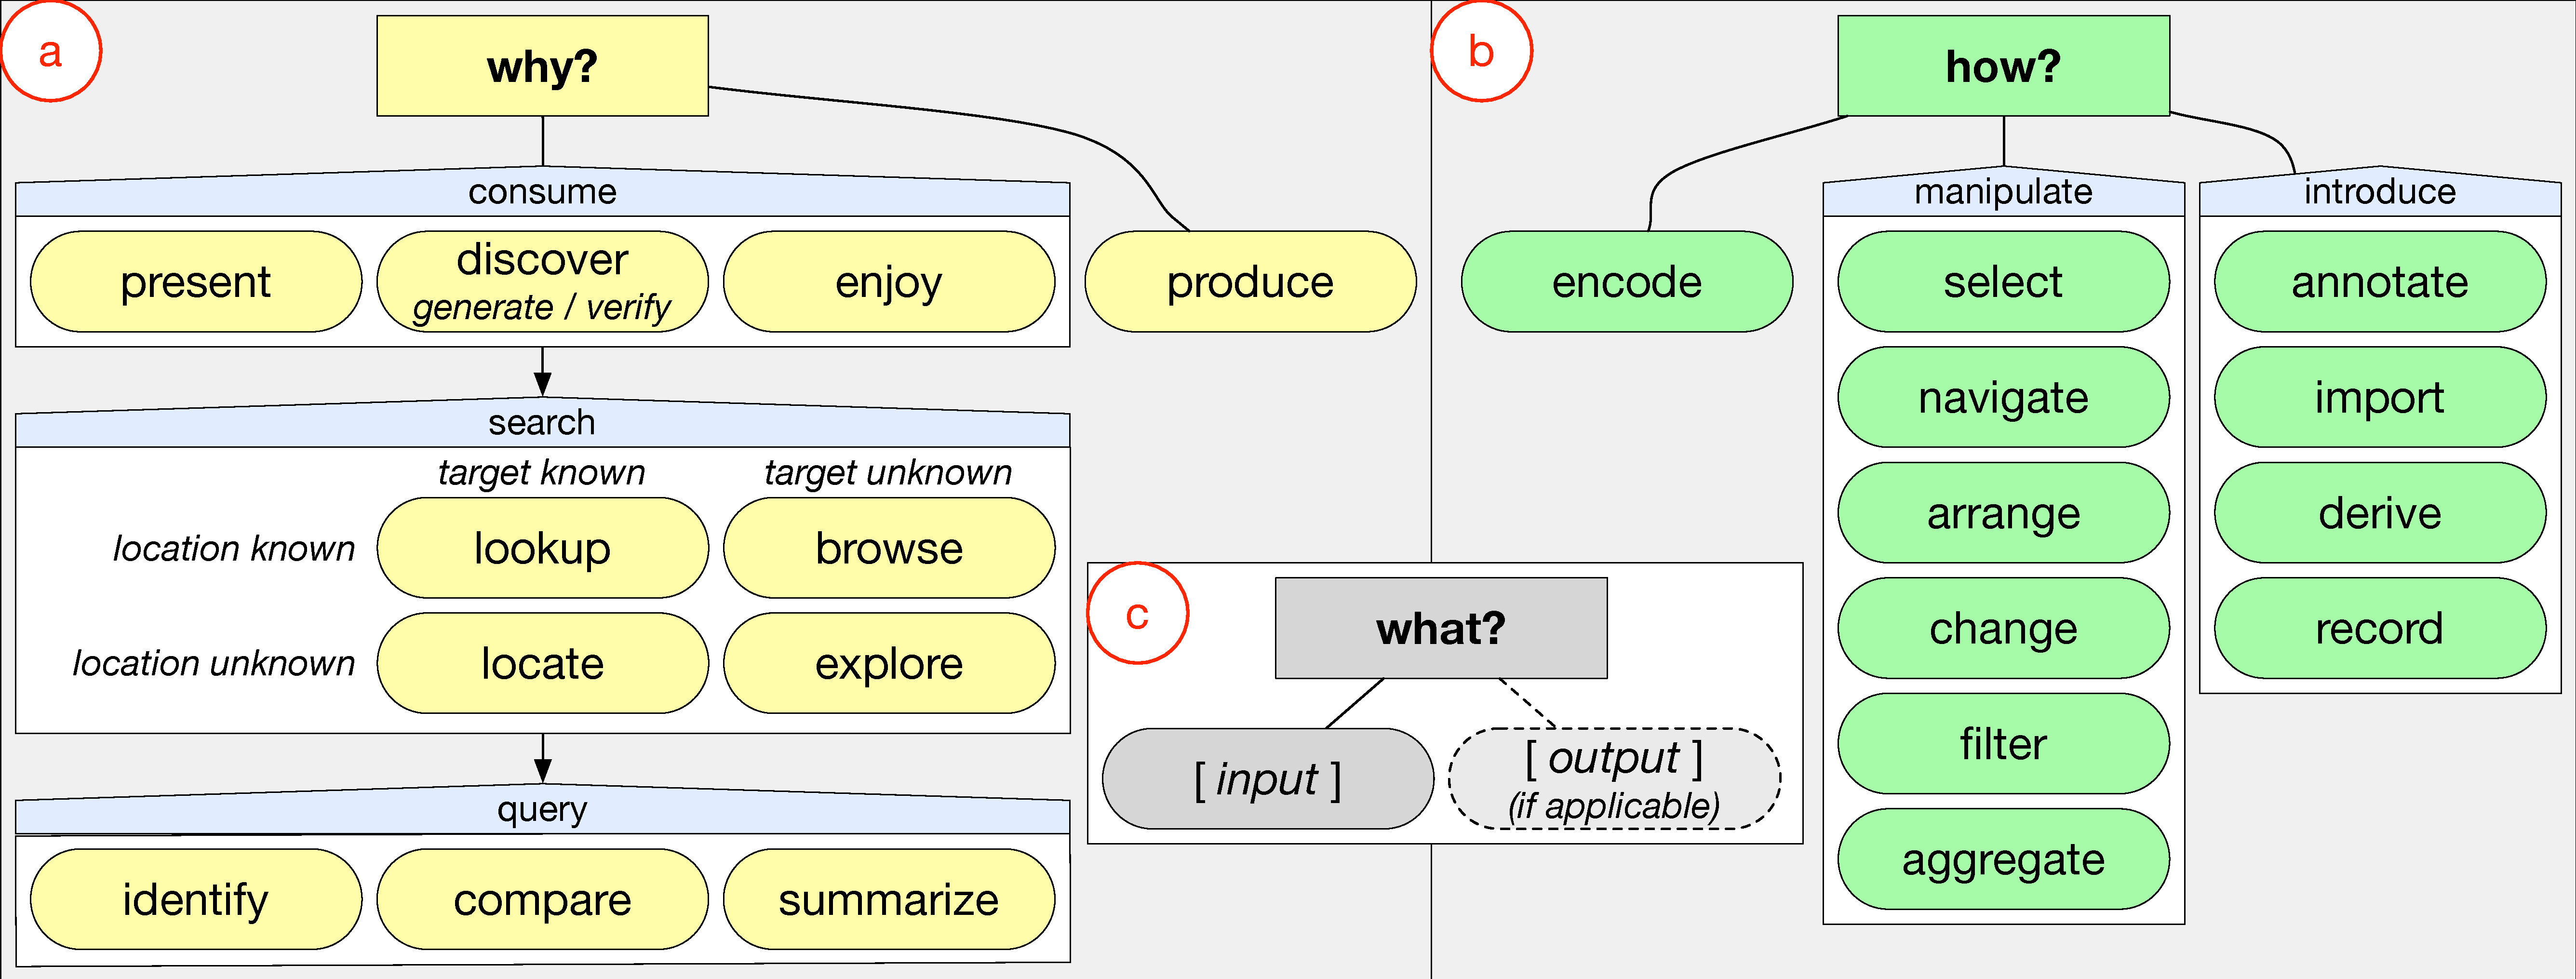
\includegraphics[width=\textwidth]{figures/typology.pdf}
    \caption
    [
        Our multi-level typology of abstract visualization tasks.
    ]
    {
        Our multi-level typology of abstract visualization tasks, which classifies  (a) {\it why} data is visualized, (b) {\it how} the task is supported in terms of visual encoding and interaction design choices, and (c) {\it what} dependencies a task might have. Note that the colors used for {\it why} and {\it how} correspond to the abstraction and technique design levels of Munzner's nested model~\cite{Munzner2009}, shown in \autoref{fig:nested-model}.
    }
    \centering
	\label{fig:typology}
\end{figure}

%-|-|-|-|-|-|-|-|-|-|-|-|-|-|-|-|-|-|-|-|-|-|-|-|-|-|-|-|-|-|-|-|-|-|-|-|-

%-|-|-|-|-|-|-|-|-|-|-|-|-|-|-|-|-|-|-|-|-|-|-|-|-|-|-|-|-|-|-|-|-|-|-|-|-

\begin{figure}
    \centering
    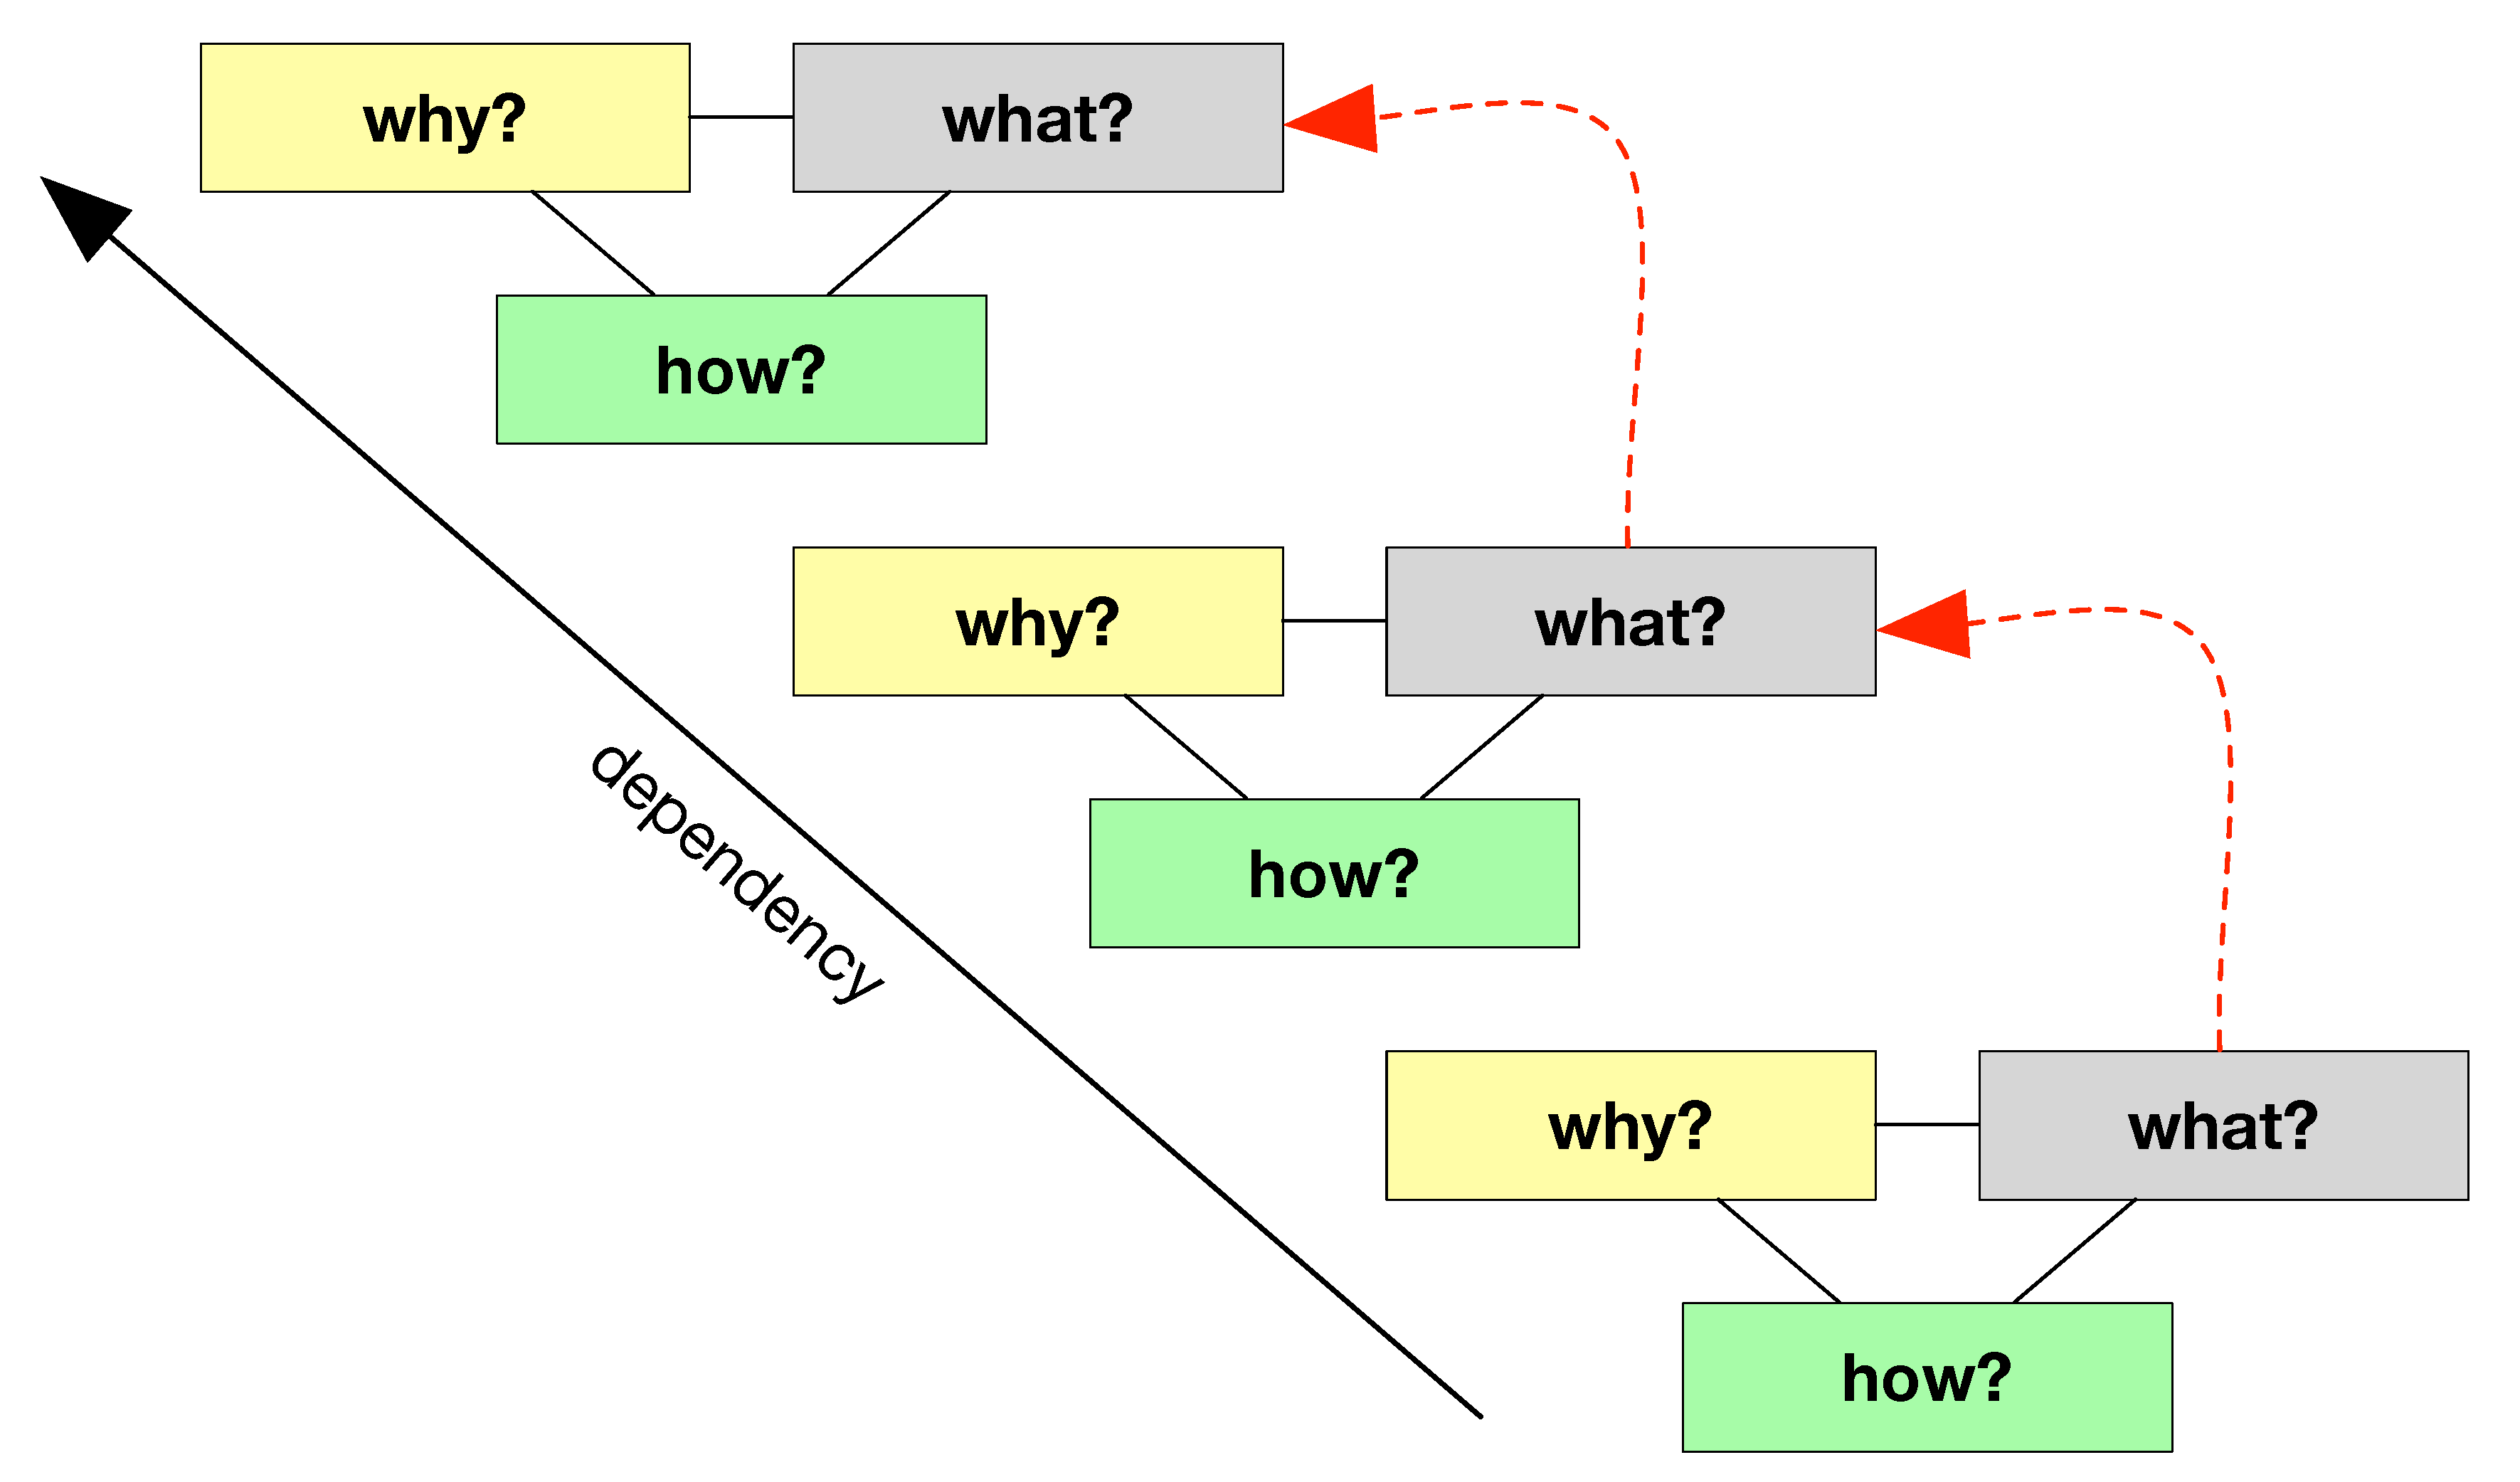
\includegraphics[width=0.75\textwidth]{figures/typology-dependency-eps-converted-to.pdf}
    \caption
    [
        Concise task descriptions using elements of the typology.
    ]{
        Concise task descriptions are constructed using elements from each part of the typology. In specifying the input and output of tasks, we can describe sequences of interdependent tasks.
    }
    \centering
    \label{fig:typology-dep}
\end{figure}

%-|-|-|-|-|-|-|-|-|-|-|-|-|-|-|-|-|-|-|-|-|-|-|-|-|-|-|-|-|-|-|-|-|-|-|-|-

%-|-|-|-|-|-|-|-|-|-|-|-|-|-|-|-|-|-|-|-|-|-|-|-|-|-|-|-|-|-|-|-|-|-|-|-|-

\begin{figure}
    \centering
    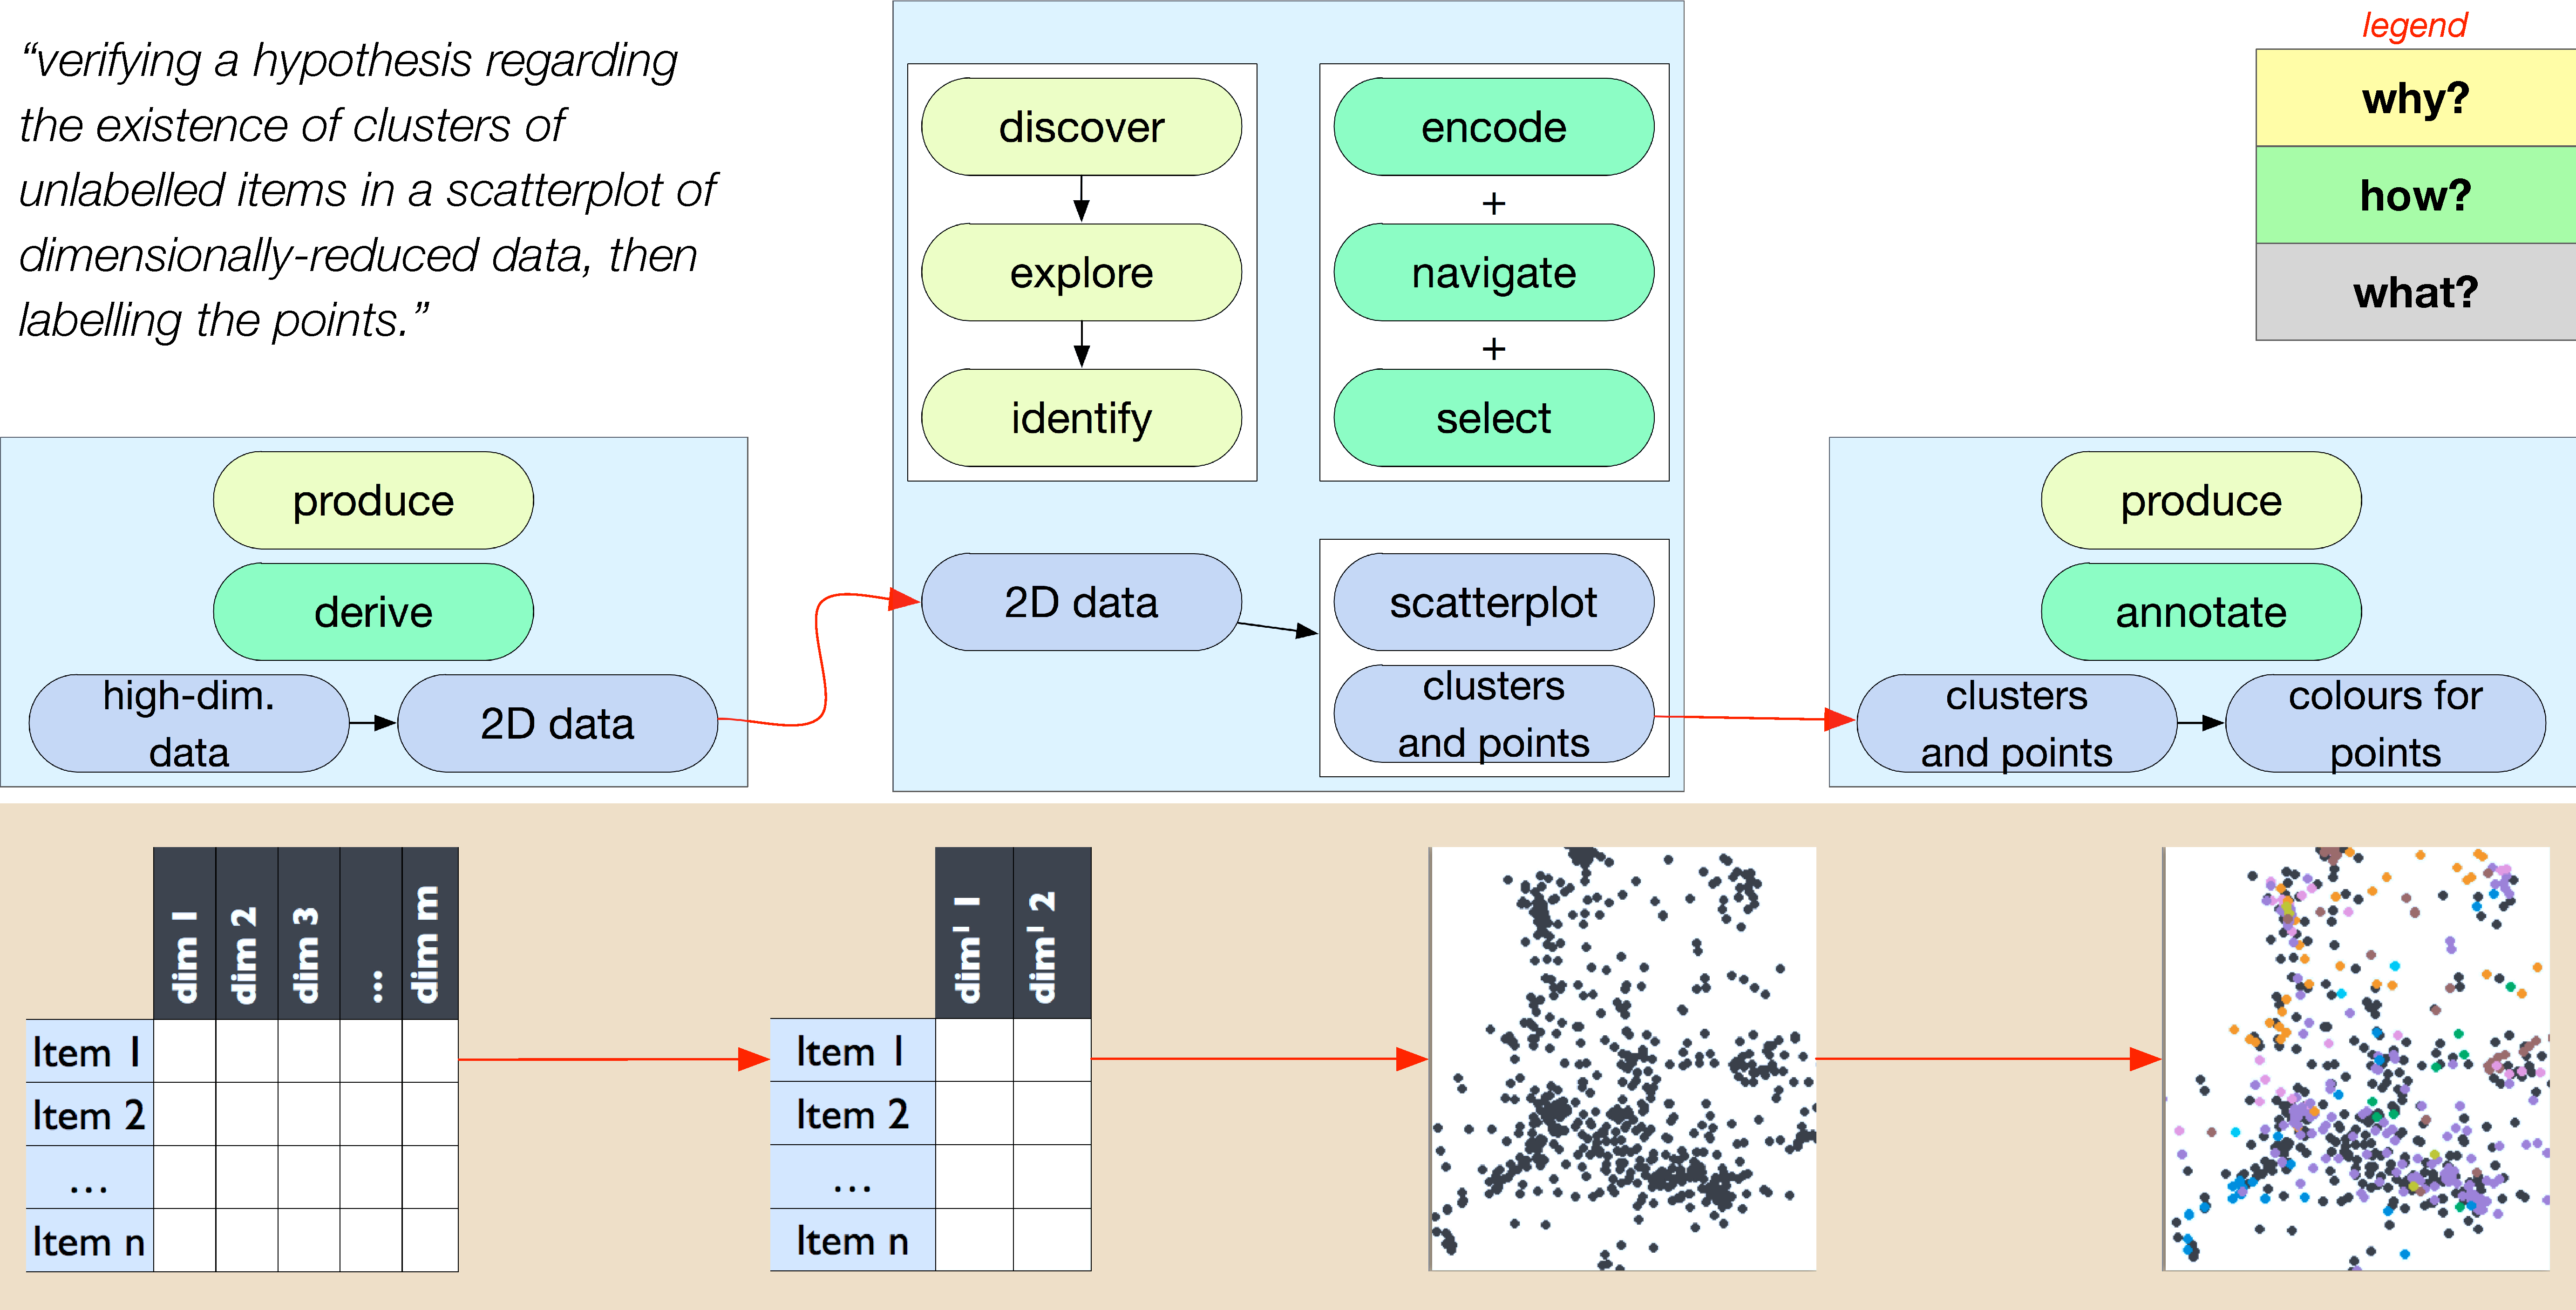
\includegraphics[width=\textwidth]{figures/typology-example-eps-converted-to.pdf}
    \caption
    [
        An example sequence of tasks using the structure and vocabulary of our typology.
    ]
    {
        An example sequence of tasks, described as a sentence (top left), as well as using the structure and vocabulary of our typology (top); the bottom depicts a series of transformations corresponding to the inputs and outputs of each task. This particular series of abstract tasks is relevant to both the interview study (\autoref{ch:drvistasks}) and field study (\autoref{ch:overview}) projects, as they both involve high-dimensional data, dimensionality reduction, and the visualization of dimensionally reduced data.
    }
    \centering
    \label{fig:typology-example}
\end{figure}

%-|-|-|-|-|-|-|-|-|-|-|-|-|-|-|-|-|-|-|-|-|-|-|-|-|-|-|-|-|-|-|-|-|-|-|-|-

%-------------------------------------------------------------------------

\subsection{Use of the Typology in an Interview Study}
\label{intro:p2}

%-------------------------------------------------------------------------

In \autoref{ch:drvistasks}, we used our typology\index{task!task typology} to {\it analyze} data analysis and the use of visualization techniques and tools ``in the wild''\index{evaluation!in the wild} by way of an interview study.
In particular, we used the typology\index{task!task typology} to examine the data analysis tasks\index{task} of individuals working in several different domains, and specifically tasks\index{task} related to the analysis of high-dimensional data\index{high-dimensional data}; we sought to better understand this data, the \ac{DR}\index{dimensionality reduction (DR)} transformations applied to it, as well as {\it why}\index{{\tt why}} and {\it how}\index{{\tt how}} visualization techniques and tools are used throughout analysts' domain-specific workflows\index{workflows}.

\bstart{Methodology}
The focus of this research was to classify the tasks associated with the visualization of dimensionally reduced data\index{dimensionality reduction (DR)}, such as in the example of \autoref{fig:typology-example}.
Our data collection and analysis methodology included twenty-four interviews with researchers and a literature survey spanning several application domains, including \ac{HCI}\index{human-computer interaction (HCI)}, chemistry\index{chemistry}, bioinformatics\index{bioinformatics}, computer science, and policy analysis\index{policy analysis}.
Our approach was similar to an interview study by \citet{Kandel2012}, one classifying data analysis and visualization among enterprise data analysts; we view our work as being complementary to their findings, given that both projects addressed data analysis and visualization ``in the wild''\index{evaluation!in the wild} for a broad group of domains.
We collected a large amount of data: diagrams, screen shots, interview notes, recordings, and transcripts, as well as interviewees' research papers, their data, and other research artifacts.

Using a qualitative coding\index{coding (qualitative data analysis)} approach, we developed a classification of task sequences\index{task!task sequence} relating to visualizing dimensionally reduced data\index{dimensionality reduction (DR)}, which are illustrated in \autoref{fig:dritw}, where each sequence\index{task!task sequence} is comprised of tasks, and each task can be defined using the vocabulary of our task typology\index{task!task typology}.
We distinguished between tasks\index{task} relating to learning about the synthetic dimensions resulting from \ac{DR} and those relating to learning about clusters of items in the dimensionally reduced data\index{dimensionality reduction (DR)}.

%-|-|-|-|-|-|-|-|-|-|-|-|-|-|-|-|-|-|-|-|-|-|-|-|-|-|-|-|-|-|-|-|-|-|-|-|-

\begin{figure}
	\centering
	\begin{subfigure}[t]{\textwidth}
	    \centering
        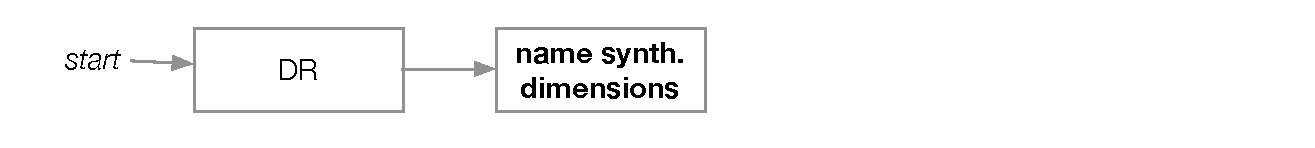
\includegraphics[height=1cm]{figures/drviztasks-name-dims.eps}
    \end{subfigure}
    ~
    \begin{subfigure}[t]{\textwidth}
	    \centering
        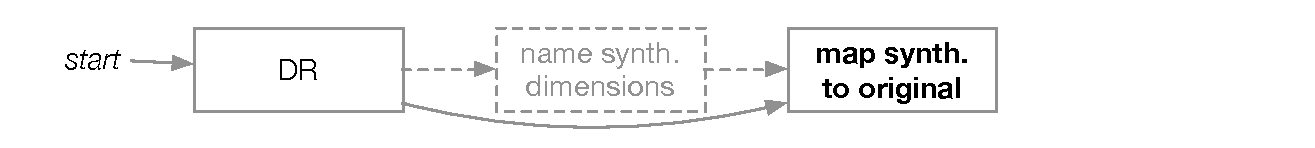
\includegraphics[height=1cm]{figures/drviztasks-map-dims.eps}
    \end{subfigure}
    ~
    \begin{subfigure}[t]{\textwidth}
	    \centering
        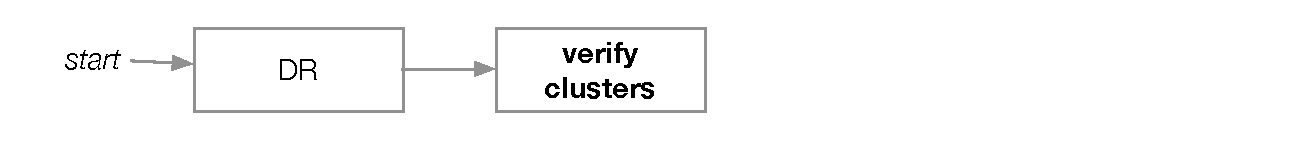
\includegraphics[height=1cm]{figures/drviztasks-identify-clusters.eps}
    \end{subfigure}
    ~
    \begin{subfigure}[t]{\textwidth}
	    \centering
        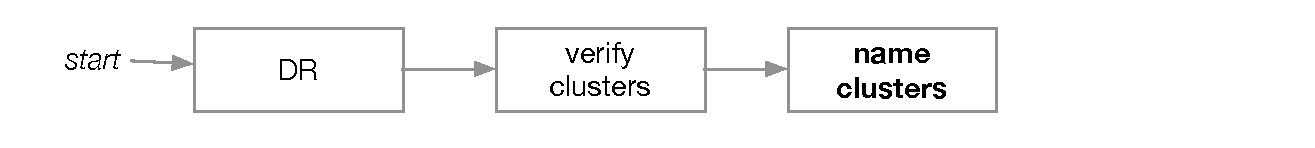
\includegraphics[height=1cm]{figures/drviztasks-name-clusters.eps}
    \end{subfigure}
    ~
    \begin{subfigure}[t]{\textwidth}
	    \centering
        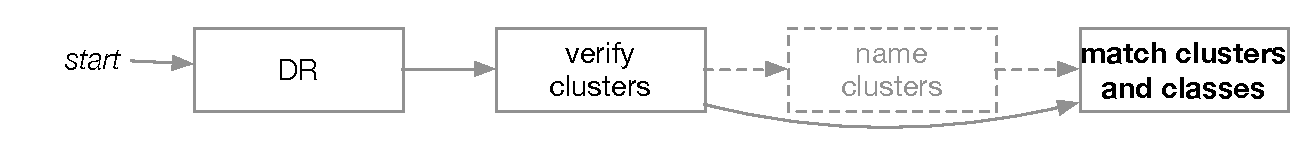
\includegraphics[height=1cm]{figures/drviztasks-match-clusters.eps}
    \end{subfigure}
	\caption
	[
	    Task sequences that involve visualizing dimensionally reduced data.
	]{
    	A classification of five task sequences that involve visualizing dimensionally reduced data, based upon findings from an interview study, documented in \autoref{ch:drvistasks}.
	}
	\centering
	\label{fig:dritw}
\end{figure}

%-|-|-|-|-|-|-|-|-|-|-|-|-|-|-|-|-|-|-|-|-|-|-|-|-|-|-|-|-|-|-|-|-|-|-|-|-

\bstart{Contributions}
With the advent of the task typology\index{task!task typology} proposed in \autoref{ch:typology}, we had a theoretical lens and vocabulary with which to approach the considerable amount of data that we collected from our interview study. 
Using the vocabulary of our typology\index{task!task typology}, %our earlier focus on dimensionality reduction can now be described using the {\it how} branch of our typology, with terms such as {\it filter}, {\it aggregate}, {\it derive}, {\it select}, and {\it annotate}. 
we were able to classify {\it why}\index{{\tt why}} these techniques are applied in sequential workflows\index{workflows}, as well as {\it what}\index{{\tt what}} the {\it inputs}\index{{\tt input}} and {\it outputs}\index{{\tt output}} of these tasks are.

\begin{sloppypar}
We contribute a {\it datatype-specific} classification of tasks grounded in observations of real-world analyst behaviour.
We encourage the further classification of tasks specific to datatype, as these are complementary to our datatype-agnostic typology\index{task!task typology} that we introduce in \autoref{ch:typology}; examples in the literature include the often-cited task by datatype taxonomy by \citet{Shneiderman1996}, classifications of graph-specific tasks~\cite{Lee2006,Saket2014}, tabular data~\cite{Henry2006}, and time-oriented data~\cite{Lammarsch2012}.
When the paper about our interview study was first published, there was no prior classification of tasks relating to visualizing dimensionally reduced data\footnote{A 2015 task taxonomy by \citet{Etemadpour2015} is discussed in \autoref{conclusions:drvistasks}.}\index{dimensionality reduction (DR)}.
The findings of our interview study and our classification of tasks is further contextualized with references to specific visual encoding\index{visual encoding} design choices; as a result, our classification of tasks can serve to validate and inform visualization technique research, a challenge that we identified in previous work~\cite{Ingram2010}.
\end{sloppypar}

%-------------------------------------------------------------------------

\subsection{Use of the Typology in a Field Study}
\label{intro:p3}

%-------------------------------------------------------------------------

In 2010, our research group began collaborating with a professional journalist who was developing a visualization tool intended for the exploration\index{{\tt explore}} of large text document collections\index{document data}.
Since this time, the tool has been deployed as {\it Overview}\footnote{\url{https://www.overviewdocs.com/}} (shown in \autoref{fig:overview}), a web-based application for investigative journalists\index{journalism} who report on large document collections\index{document data} attained from \ac{FOIA} requests or from whistleblower organizations, collections ranging in size from hundreds to tens of thousands of documents.
Between 2012 and 2014, we conducted a post-deployment field study evaluation of {\it Overview}\index{Overview (document mining tool)}, in which we analyzed its adoption\index{adoption} and self-initiated use by investigative journalists.
\autoref{ch:overview} documents this field study.

%-|-|-|-|-|-|-|-|-|-|-|-|-|-|-|-|-|-|-|-|-|-|-|-|-|-|-|-|-|-|-|-|-|-|-|-|-

\begin{figure}
    \centering
    \fbox{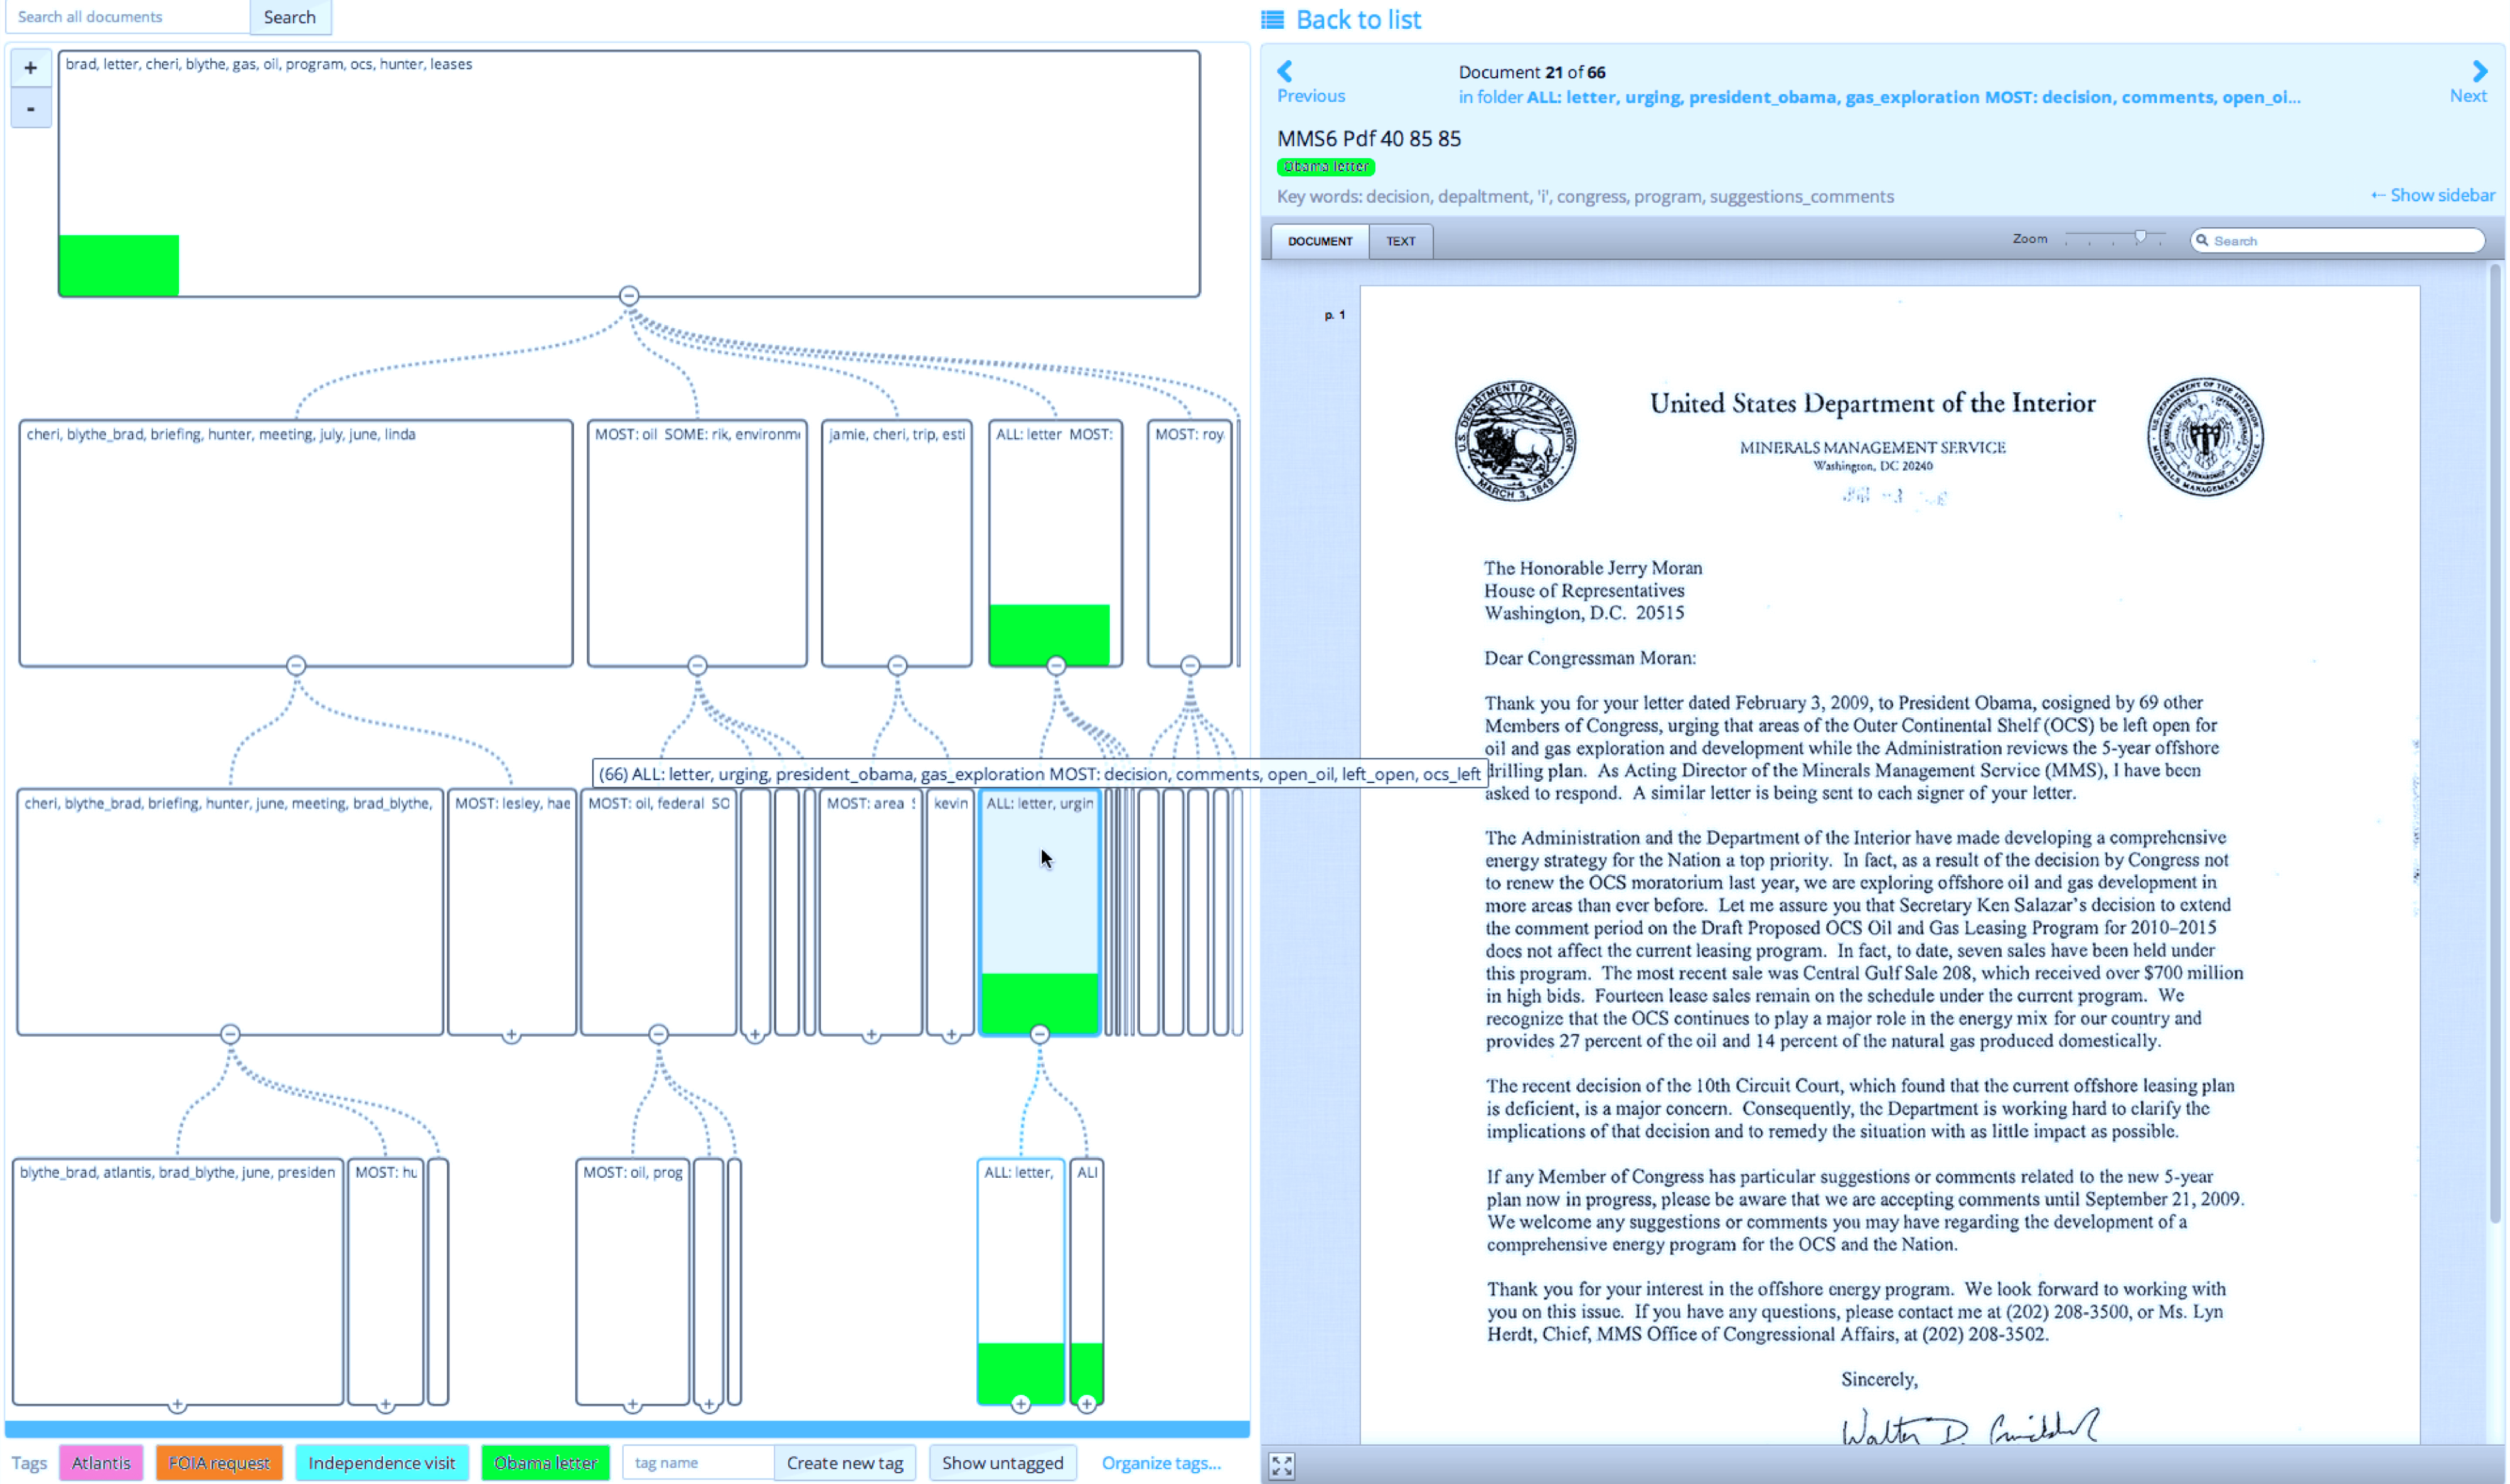
\includegraphics[width=0.975\textwidth]{figures/overview-v4-eps-converted-to.pdf}}
    \caption
    [
        {\it Overview}, a multiple-view application intended for use during an investigation of a large collection of text documents.
    ]{
        {\it Overview} is a multiple-view application intended for the systematic search, annotation, and reading of a large collection of text documents, which visualizes hierarchical clusters of documents as a tree (left). 
    }
    \centering
    \label{fig:overview}
\end{figure}

%-|-|-|-|-|-|-|-|-|-|-|-|-|-|-|-|-|-|-|-|-|-|-|-|-|-|-|-|-|-|-|-|-|-|-|-|-

\bstart{Methodology}
We conducted case studies\index{case study} of six journalists who used {\it Overview}\index{Overview (document mining tool)} to conduct investigations involving large document collections\index{document data}; in five of these cases, the investigation resulted in a published story, and one of these stories~\cite{Playford2013} was a finalist for the 2014 Pulitzer Prize in journalism\footnote{\url{http://www.pulitzer.org/2014_public_service_finalist}}.
A critical difference between our approach and other post-deployment field studies that focus on the usage of visualization tools or techniques~\cite{Lloyd2011,Saraiya2006,Shneiderman2006} is that our case study\index{case study} participants were not solicited by the researchers: they freely chose to use {\it Overview}\index{Overview (document mining tool)} and they did not inform preceding phases of design. 
We also engaged a different set of people at each stage of design, rather than the same set of people. 
This difference reflects {\it Overview}'s\index{Overview (document mining tool)} context of use: repeat usage cannot be predicted and {\it Overview}\index{Overview (document mining tool)} is only appropriate for some investigations; we have yet to encounter a journalist who specializes in investigations pertaining to large document collections\index{document data}.

We interviewed these six journalists about the form and provenance of their documents\index{document data}, the objectives of their investigation, and their use of {\it Overview}; we also collected their logged interaction data and their annotated\index{{\tt annotate}} document collections\index{document data}.
We used our task typology\index{task!task typology}, which we introduce in \autoref{ch:typology}, to better understand {\it why}\index{{\tt why}} {\it Overview}\index{Overview (document mining tool)} was adopted by these journalists to perform their investigations.

\bstart{Results}
The analysis of journalists' use of {\it Overview}\index{Overview (document mining tool)} revealed that our initial understanding of their task\index{task} was insufficient: the task\index{task} of {\it ``exploring''}\index{{\tt explore}} a document collection\index{document data}, a term that appears often in previous work on visualizing document data, is both too vague and too narrow to capture how journalists actually used {\it Overview}\index{Overview (document mining tool)}. 
% RR: p. 3. "exploring [234] or integrating insights [188] are quite abstract". Do you really mean "abstract", or do you mean "vague"? (cf. discussion of "exploring" on p. 11.) Related to this: couldn't "finding an extreme value" be abstract?  If not, what do you mean by "abstraction"? Isn't this simply independence of the details of the task?
Instead, we identified two different tasks\index{task} using the vocabulary and structure of our typology\index{task!task typology}: one of {\it generating}\index{{\tt discover}} hypotheses and {\it summarizing}\index{{\tt summarize}} the contents of a document collection, and another of {\it locating}\index{{\tt locate}} and {\it identifying}\index{{\tt identify}} specific evidence in order to {\it verify}\index{{\tt discover}} or {\it refute} prior hypotheses.

\bstart{Contributions}
Given our more precise understanding of journalists' tasks, we were able to rigorously analyze the rationale for {\it Overview}'s\index{Overview (document mining tool)} visual encoding\index{visual encoding} and interaction\index{interaction} design choices.
This analysis is transferable beyond the domain of journalism\index{journalism} and speaks to the design of visualization techniques and tools addressing document data\index{document data} and to some extent any data that can be hierarchically structured\index{hierarchical data}.
% In addition, our analysis of real world visualization usage is a form of validation for our task typology~\cite{Brehmer2013}.
Finally, we reflect upon {\it Overview}'s\index{Overview (document mining tool)} design and evaluation process, comparing our approach to previous human-centred visualization design processes~\cite{Isenberg2008,Lloyd2011}; we also discuss the value, logistics, and limitations of studying the adoption\index{adoption} of visualization techniques or tools.

%-------------------------------------------------------------------------

\subsection{Use of the Typology in a Design Study}
\label{intro:p4}

%-------------------------------------------------------------------------

In 2013, we initiated a visualization design study\index{design studies} project that provided an opportunity to validate the {\it generative} potential of our typology\index{task!task typology}.
This project was a collaboration with a company that develops energy\index{energy management} usage reporting software for multi-building organizations such as universities, school boards, or hotel chains.
Many of these client organizations have designated energy analysts who oversee large portfolios of buildings; these analysts are responsible for identifying\index{{\tt identify}} cost saving opportunities, diagnosing erratic energy usage behaviour, and attempting to understand the role of fluctuating external factors such as weather, occupancy, operating hours, and equipment usage within buildings.
Tools and techniques for addressing these tasks with respect to single buildings already exist, however they do not scale to portfolios of dozens or hundreds of buildings.
% In addition, many commercial buildings are now outfitted to report energy usage at the granularity of minutes, rather than months, which is still typical of residential buildings.
We conjectured that an interactive application integrating visualization while considering these issues of scale could address the tasks\index{task} of these analysts.
\autoref{ch:emu} documents this design study.
% A recent design study~\cite{Goodwin2013} successfully applied visualization techniques to the analysis of  modelling residential energy usage for thousands of households, which gave us hope that visualization techniques could also be applied to the analysis of large commercial building portfolios.

\bstart{Methodology}
We began by analyzing the energy domain and interviewing energy analysts from commercial client organizations who had previously used our industry partner's software, asking them about their roles and responsibilities, their technical background, their portfolio of buildings, and the limitations of current tools.
We also presented our interview findings and sought additional feedback from members of our industry partner's client services team, who have expertise with the current software and act as liaisons to client organizations.

Once again, we used our task typology\index{task!task typology}, to identify and abstract the tasks\index{task!task abstraction} of these analysts.
We narrowed our scope to tasks\index{task} that recurred often among the analysts and those that were consistent with the mandate of our industry partner's product development team to support analysis of energy consumption in building portfolios.

Over the course of four months, we designed and implemented over a dozen interactive visualization {\it data sketches}~\cite{Lloyd2011}\index{data sketch} to address the tasks\index{task} of these analysts, following a process of rapid iteration in which functional sketches featuring the analysts' data were used to further refine our understanding of their tasks\index{task} and context of use.
These data sketches\index{data sketch} were produced within the interactive interactive sandbox environment shown in \autoref{fig:pulse-cal}.
Our task abstractions\index{task!task abstraction} informed the process of mapping these tasks to a set of appropriate visual encoding\index{visual encoding} and interaction\index{interaction} design choices.
The design choices that we considered included those for performing multiple comparisons\index{{\tt compare}} between aggregate and individual items over time~\cite{Aigner2011}, for identifying\index{{\tt identify}} cyclic and acyclic events using meaningful temporal granularities~\cite{VanWijk1999}, and for identifying\index{{\tt identify}} differences in multiple lists of ranked items while simultaneously identifying the cause of rank changes~\cite{Gratzl2013}.

In early 2014, we conducted {\it chauffeured demos}~\cite{Lloyd2011}\index{chauffeured demos} of these interactive data sketches\index{data sketch} with four groups of analysts; the energy usage data used in these demos was collected from analysts' own building portfolios. 
By integrating the feedback we received on our sketches\index{data sketch} and our understanding of energy analysts' tasks\index{task}, we then envisioned ways to juxtapose\index{view coordination!view juxtaposition} and sequence\index{view coordination!view sequencing} discrete {\it views}\index{view coordination} of the data in order to support workflows\index{workflows}, and we continued to elicit feedback from analysts and our collaborators' client services team.

%-|-|-|-|-|-|-|-|-|-|-|-|-|-|-|-|-|-|-|-|-|-|-|-|-|-|-|-|-|-|-|-|-|-|-|-|-

\begin{figure}
    \centering
    \fbox{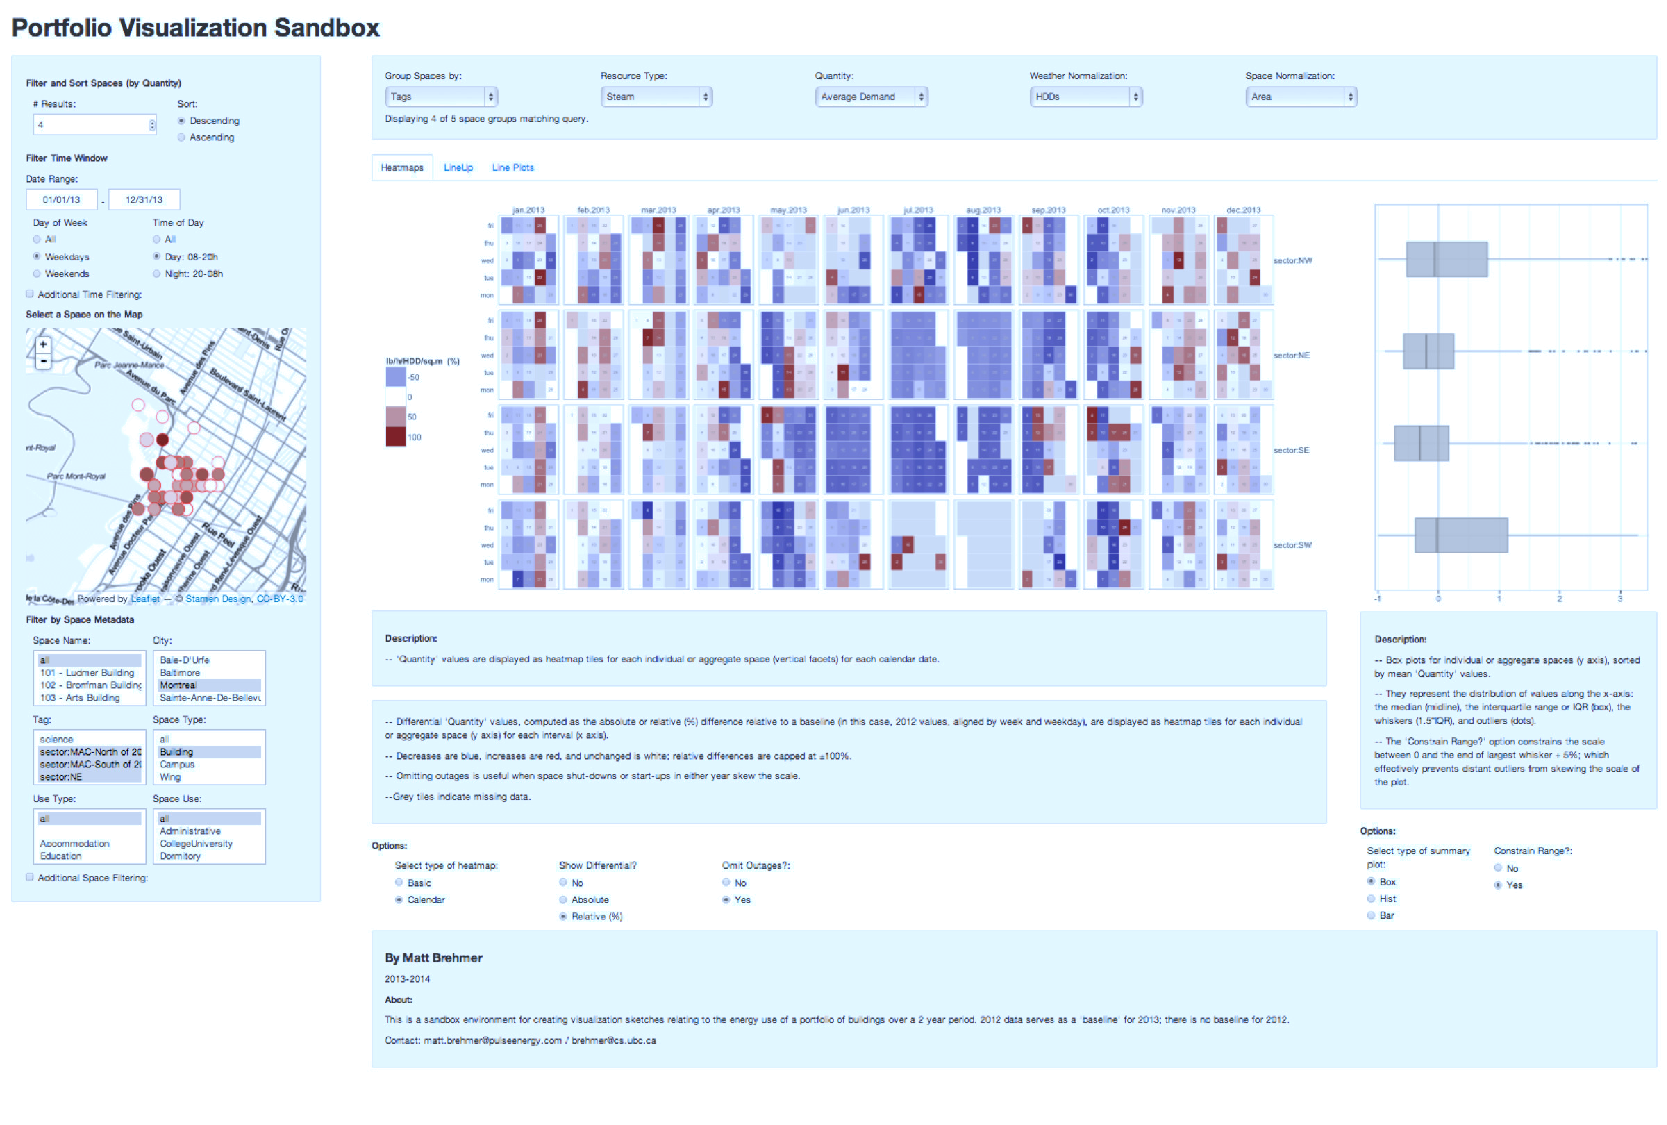
\includegraphics[width=0.975\textwidth]{figures/pulse-cal-eps-converted-to.pdf}}
    \caption
    [
         A sandbox environment for creating visualization data sketches pertaining to energy portfolio analysis.
    ]{
        A sandbox environment for creating visualization data sketches pertaining to the analysis of energy usage in large building portfolios. In this visualization data sketch, a calendar-based time series matrix is juxtaposed with summary boxplots, where each row is a group of buildings. Both the matrix and the boxplots encode the difference between average energy demand in 2012 and 2013.
    }
    \label{fig:pulse-cal}
    \centering
\end{figure}

%-|-|-|-|-|-|-|-|-|-|-|-|-|-|-|-|-|-|-|-|-|-|-|-|-|-|-|-|-|-|-|-|-|-|-|-|-

\bstart{Results}
Our collaborators have since adopted\index{adoption} a number of our designs into a new version of their commercial energy analysis software tool.
They assigned over ten full-time software developers to the project since mid-2014 and the tool has since been released to some client organizations in a small pilot deployment; the tool will soon\footnote{Relative to November 2015.} be deployed to thousands of other clients.

\bstart{Contributions}
As a result of abstracting the data and tasks\index{task!task abstraction} relating to the energy management\index{energy management} domain, visualization practitioners working in other domains might benefit from our classification of matches and mismatches between abstract tasks\index{task!task abstraction} and visualization design choices, particularly for domains that involve comparing\index{{\tt compare}} many concurrent time series\index{time-oriented data}.

We also confronted issues of domain convention\index{domain convention} in this project; in the energy sector, some visual encodings\index{visual encoding} carry very specific meanings. 
We considered how to introduce unfamiliar\index{familiarity} visual encodings\index{visual encoding} and how to get people working in this domain to trust\index{trust} them.

Finally, we contribute some methodological guidance for visualization design studies\index{design studies}, including our approach to work domain analysis\index{work domain analysis}, a systematic task analysis\index{task!task analysis} and abstraction\index{task!task abstraction}, our sandbox prototyping and workflow\index{workflows} design, as well as how to effectively present visualization design documentation.

%-------------------------------------------------------------------------

\subsection{Summary of Contributions}
\label{intro:contrib-summary}

%-------------------------------------------------------------------------

The contributions of this dissertation can be summarized as follows:

\begin{itemize}
    \item A typology\index{task!task typology} of abstract visualization tasks\index{task}, which allows for succinct descriptions of tasks and task sequences\index{task!task sequence} in terms of {\it why}\index{{\tt why}} data is visualized, {\it what}\index{{\tt what}} dependencies a task might have in terms of {\it input}\index{{\tt input}} and {\it output}\index{{\tt output}}, and {\it how}\index{{\tt how}} the task is supported in terms of visual encoding\index{visual encoding} and interaction\index{interaction} design choices (\autoref{ch:typology}).
    \item A synthesis of the literature relating to visualization tasks\index{task} (\autoref{ch:typology}).
    \item A datatype-specific classification of five task sequences\index{task!task sequence} relating to visualizing dimensionally reduced data\index{dimensionality reduction (DR)}, one based on findings from our interview study with data analysts spanning several application domains. This classification draws upon and demonstrates the descriptive power of our typology of tasks\index{task!task typology} and is intended to inform the design of new tools and techniques for visualizing dimensionally reduced data\index{dimensionality reduction (DR)} (\autoref{ch:drvistasks}).
    \item A field study evaluation of {\it Overview}\index{Overview (document mining tool)}, a visualization tool for investigating large text document collections\index{document data}. We draw upon and demonstrate the descriptive and evaluative power of our typology of tasks\index{task!task typology} and characterized two abstract tasks relating to document mining\index{document mining} (\autoref{ch:overview}). 
    \item Seven lessons relating to the design of interactive visualization tools for hierarchical data\index{hierarchical data} and document data\index{document data} in particular. These lessons are based on an analysis of successive deployed versions of {\it Overview}\index{Overview (document mining tool)} and its adoption\index{adoption} by self-initiated journalists\index{journalism} (\autoref{ch:overview}).
    \item A methodological reflection on the study of visualization adoption\index{adoption} (\autoref{ch:overview}).
    \item A demonstration of the descriptive, evaluative, and generative power of our typology of tasks\index{task!task typology} in a visualization design study\index{design studies} within the energy domain (\autoref{ch:emu}).
    \item An identification of matches and mismatches between visualization design choices and three abstract tasks for concurrent time series data\index{time-oriented data} (\autoref{ch:emu}).
    \item Two lessons pertaining to familiarity\index{familiarity} with visual encodings\index{visual encoding}, two lessons pertaining to the trust\index{trust} of data aggregation design choices\index{{\tt aggregate}}, and three lessons pertaining to visualization design methodology (\autoref{ch:emu}).
\end{itemize}

%-------------------------------------------------------------------------
%-------------------------------------------------------------------------

\section{Extension and Impact of the Typology}
\label{intro:adoption}

%-------------------------------------------------------------------------
%-------------------------------------------------------------------------

In \autoref{ch:conclusions}, we comment on how our task typology was subsequently extended by Munzner in her 2014 book {\it Visualization Analysis and Design}~\cite{Munzner2014}; this modified typology is shown in \autoref{fig:typology-extension}.
Munzner moved {\it introduce} nodes from the {\it how} part of the typology to become forms of {\it produce} in the {\it why} part of the typology; she also added {\it targets} to the {\it why} part of the typology, referring to the original {\it why} part of our typology as {\it actions}; finally, she reorganized the {\it how} part of the typology and elaborated on forms of {\it encode}.
We explicitly make reference to and use Munzner's modifications to the typology\index{task!task typology} in our interview study  (\autoref{ch:drvistasks}) and in our design study ({\autoref{ch:emu}).
\autoref{ch:conclusions} also contains commentary on the origin, the benefits, and the potential drawbacks of Munzner's modifications.

We also present a survey of how our task typology\index{task!task typology} and our approach to systematically analyzing and abstracting tasks has been used and/or extended by others in the visualization community, including how our typology\index{task!task typology} may integrate with novel theoretical frameworks.
This survey includes the use of our typology\index{task!task typology} to analyze domain-specific usage of visualization techniques or tools, from bioinformatics\index{bioinformatics} to malware analysis, as well as datatype-specific visualization usage, from geospatial data to multiplex networks.
This survey also includes the use of our typology\index{task!task typology} to specify and contextualize tasks in experimental studies, as well as the use of our typology\index{task!task typology} to motivate the design of novel visualization techniques and tools.

%-|-|-|-|-|-|-|-|-|-|-|-|-|-|-|-|-|-|-|-|-|-|-|-|-|-|-|-|-|-|-|-|-|-|-|-|-

\begin{figure}
	\centering
	\begin{subfigure}[t]{0.48\textwidth}
	    \centering
        \fbox{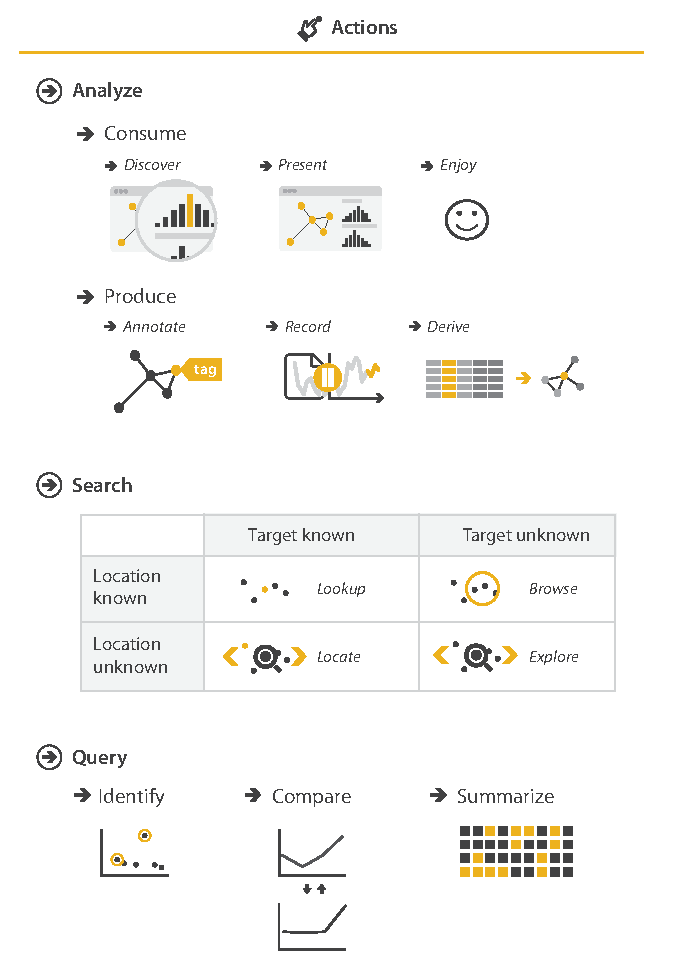
\includegraphics[height=7.75cm]{figures/fig3-2.pdf}}
        \caption{{\it why} ({\it actions}).}
    \end{subfigure}
    ~
    \begin{subfigure}[t]{0.48\textwidth}
	    \centering
        \fbox{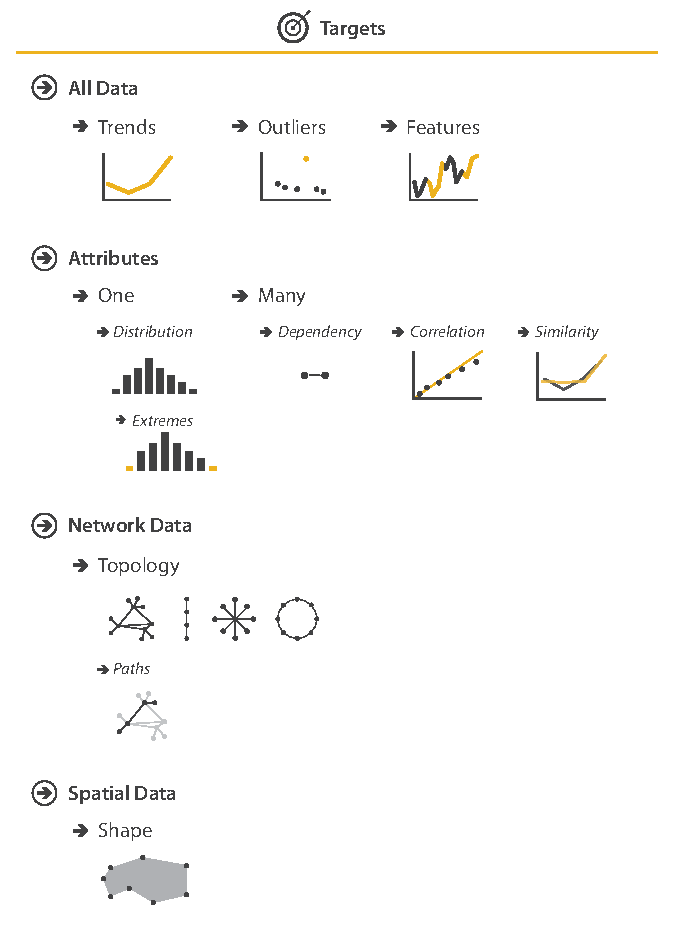
\includegraphics[height=7.75cm]{figures/fig3-6.pdf}}
        \caption{{\it why} ({\it targets}).}
    \end{subfigure}
    ~
    \begin{subfigure}[t]{\textwidth}
	    \centering
        \fbox{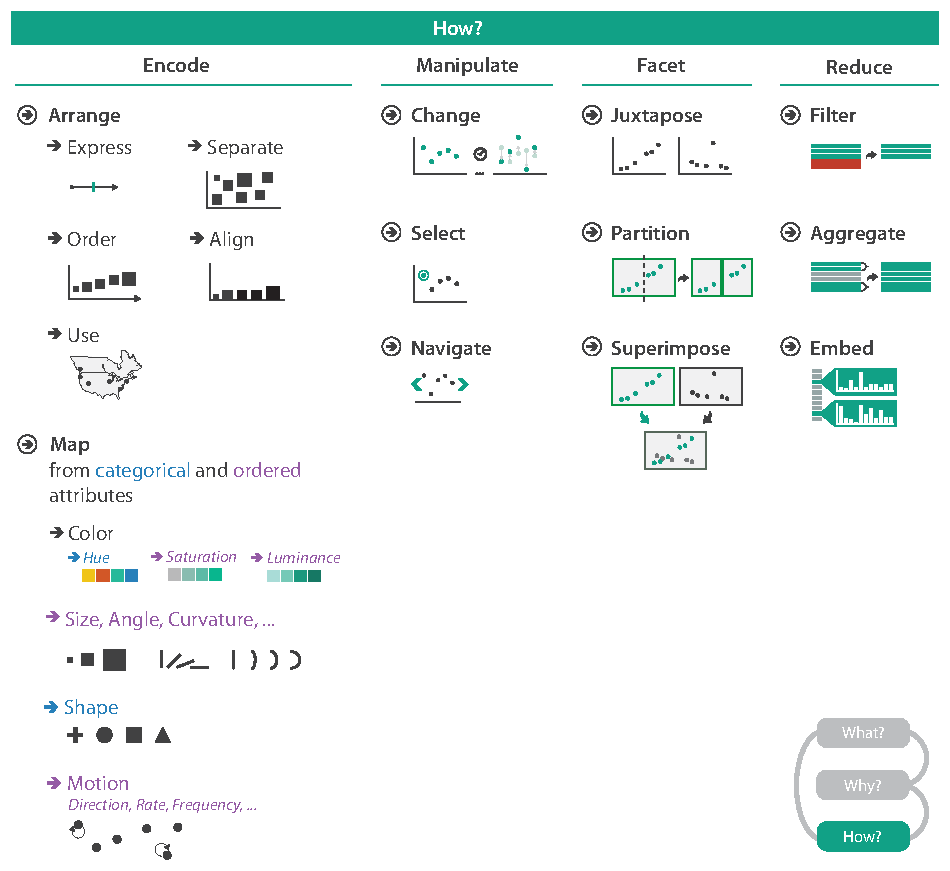
\includegraphics[height=7cm]{figures/fig3-7.pdf}}
        \caption{{\it how} (design choices).}
    \end{subfigure}
	\caption
	[
	    A modified version of our typology appearing in \citet{Munzner2014}.
	]{
    	A modified version of our typology appearing in \citet{Munzner2014} (\cf \autoref{fig:typology}): (a) forms of {\it produce} were moved from {\it how}; (b) a new classification of {\it targets}; (c) a reorganization of {\it how}. Illustrations: \ccLogo~E. Maguire (2014).
	}
	\centering
	\label{fig:typology-extension}
\end{figure}

%-|-|-|-|-|-|-|-|-|-|-|-|-|-|-|-|-|-|-|-|-|-|-|-|-|-|-|-|-|-|-|-|-|-|-|-|-

%-------------------------------------------------------------------------
%-------------------------------------------------------------------------
\section{A Note on Chronology}
\label{intro:chronology}

%-------------------------------------------------------------------------
%-------------------------------------------------------------------------

The duration of the projects described in this dissertation extended long periods of time.
As a result, periods of focused research on these projects were interleaved or overlapping.
\autoref{fig:thesis-timeline} illustrates the chronological history of these projects, indicating the core focus periods of projects, important milestones, as well as periods of part-time focus.
\autoref{fig:thesis-timeline} also indicates other milestones in my PhD, research projects not included in this dissertation~\cite{Brehmer2014a,Fulda2015}, and internships.

%-|-|-|-|-|-|-|-|-|-|-|-|-|-|-|-|-|-|-|-|-|-|-|-|-|-|-|-|-|-|-|-|-|-|-|-|-

\begin{figure}
    \centering
    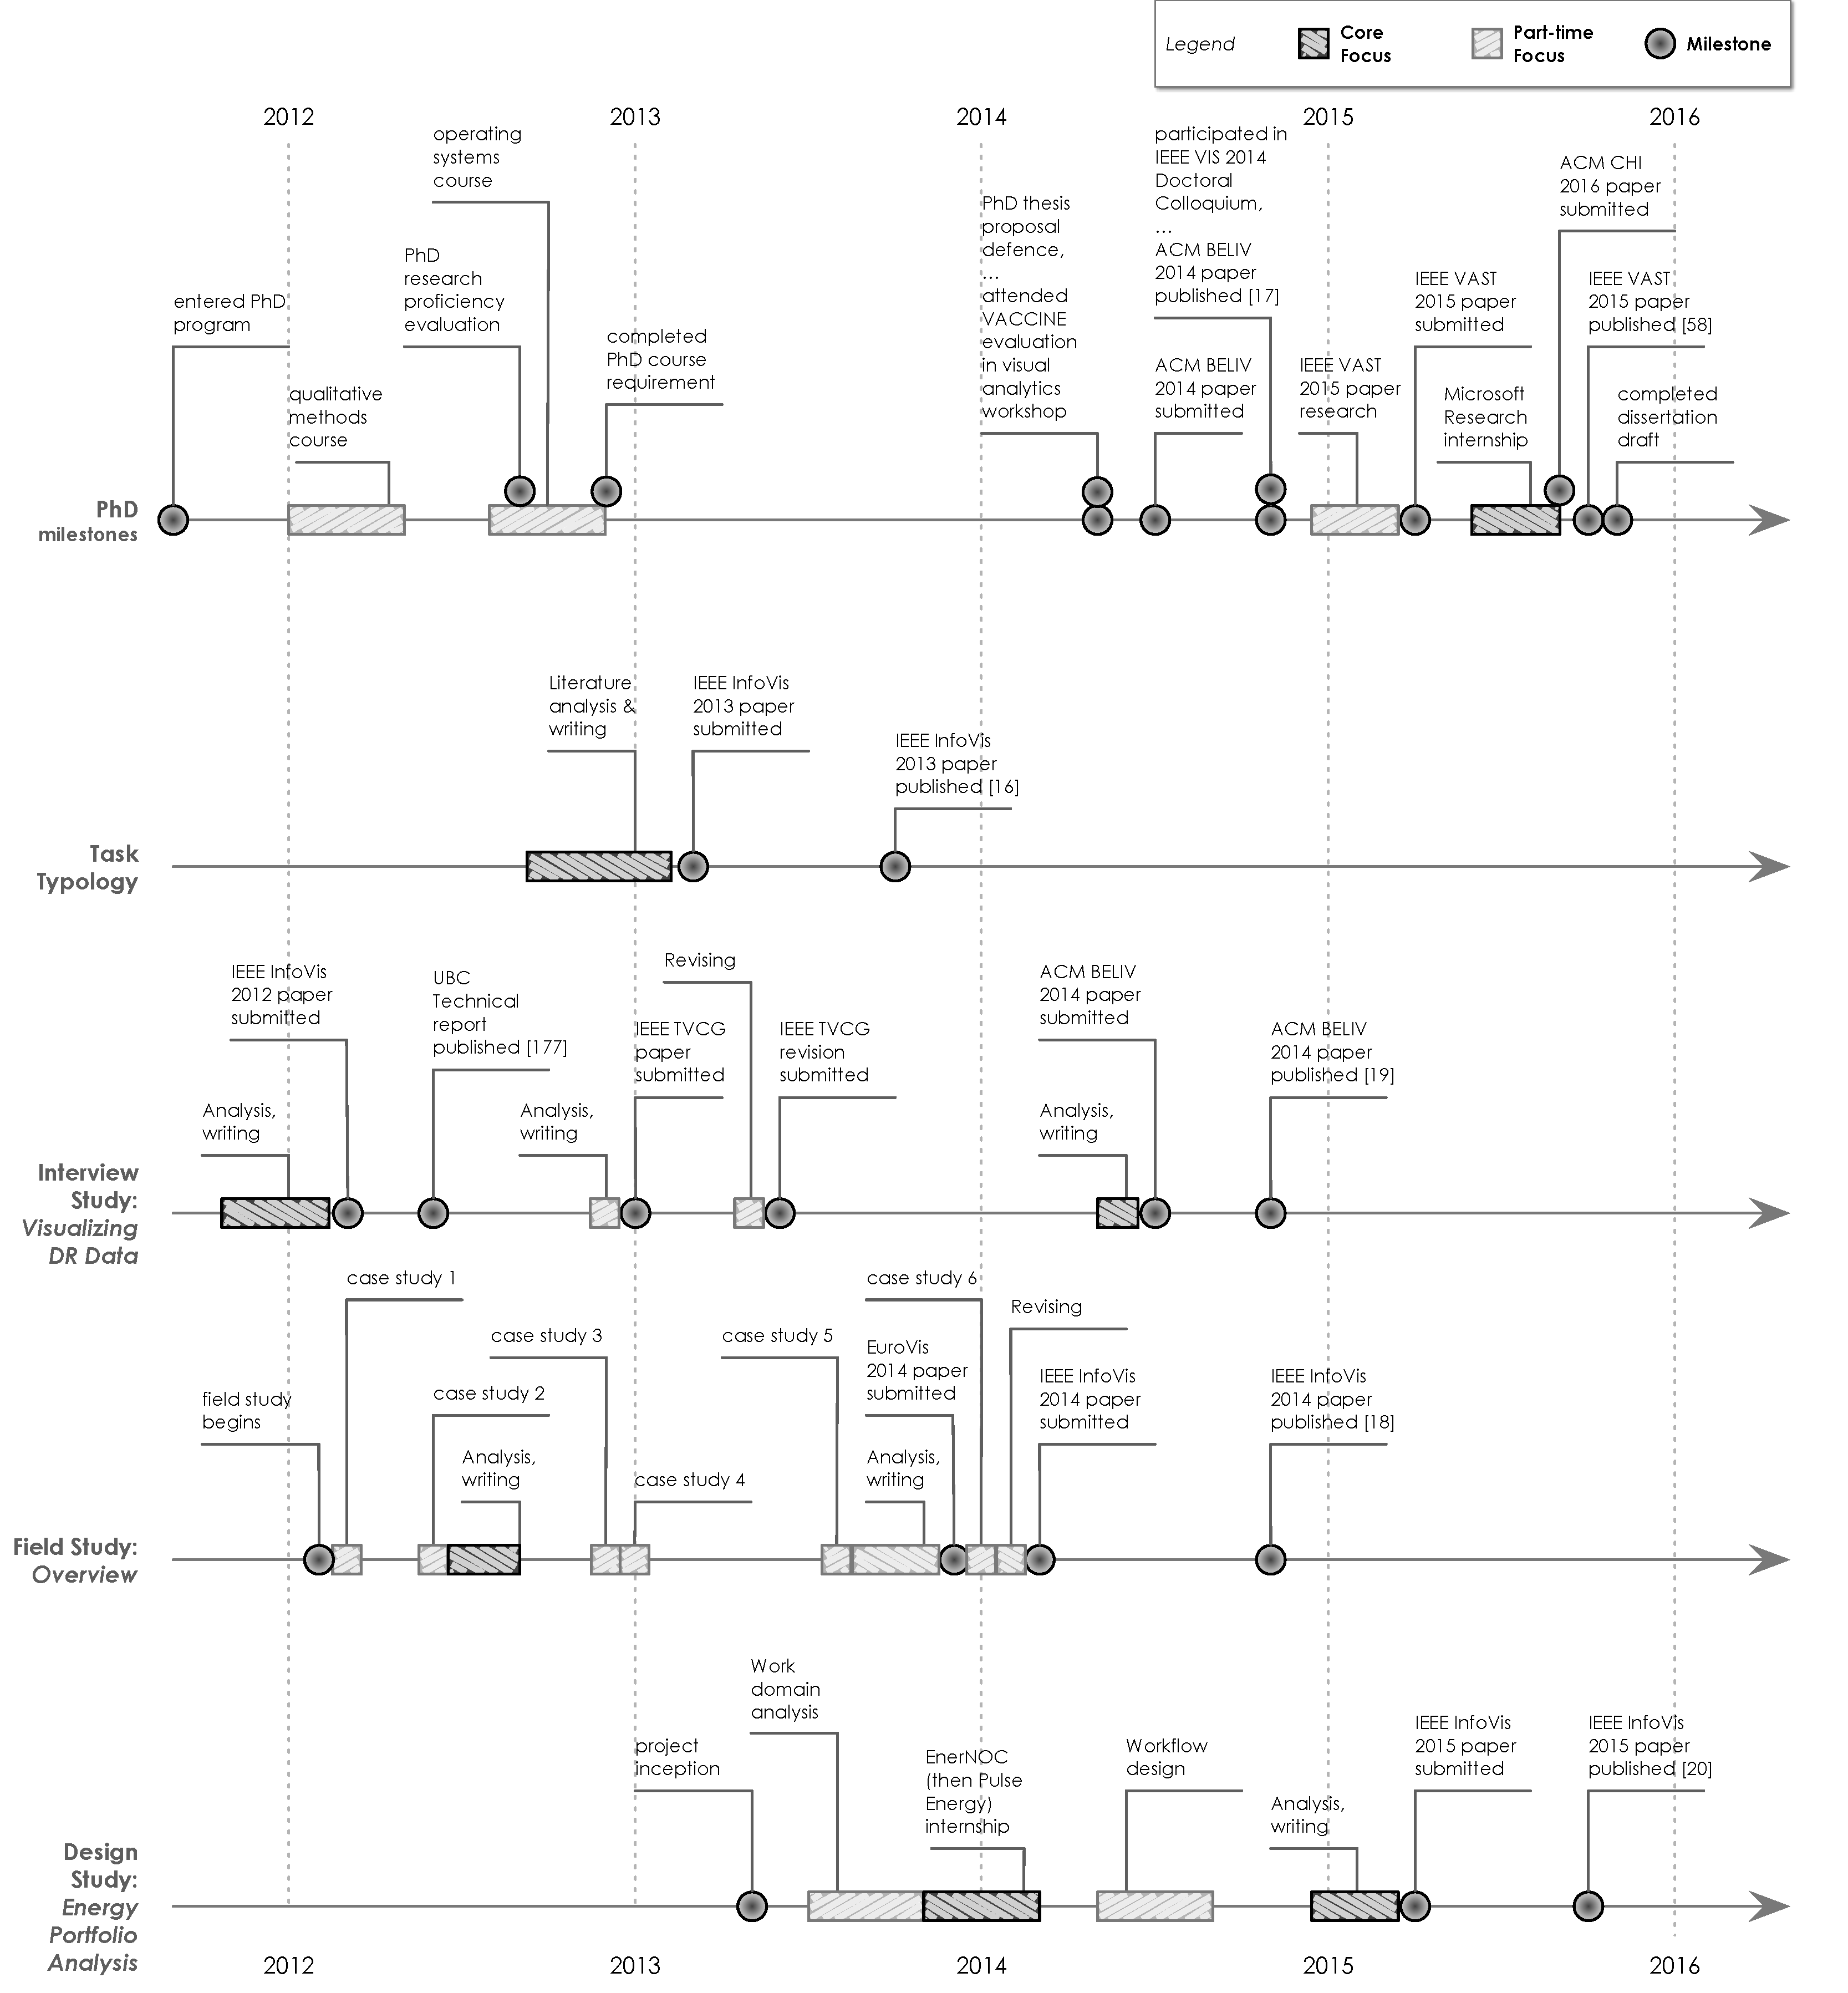
\includegraphics[width=\textwidth]{figures/thesis-timeline.pdf}
    \caption
    [
        Timelines of the projects described in this dissertation.
    ]{
        Timelines of the projects described in this dissertation. Note that the projects described in this dissertation overlapped in time. While the order of the chapters in this dissertation reflect the order in which the projects were completed, they do not reflect the order in which they were initiated.
    }
    \label{fig:thesis-timeline}
    \centering
\end{figure}

%-|-|-|-|-|-|-|-|-|-|-|-|-|-|-|-|-|-|-|-|-|-|-|-|-|-|-|-|-|-|-|-|-|-|-|-|-

\endinput
